\begin{algorithm}[t]
\DontPrintSemicolon
\caption{Hessian AWare Quantization}
\label{alg:hq}
    \SetAlgoLined
    \KwInput{Block-wise Hessian eigenvalues $\lambda_i$ (computed from~\aref{alg:power_iteration}), and block size $n_i$ 
    for $i=1,\cdots,b$.

    }

    \For(\tcp*[h]{Compute Quantization Precision}){i $=1,2,\ldots, b$}{

        $S_i = \lambda_i/n_i$ \tcp*{See~\eref{eqn:define_S}}
    }
    
    
    Order $S_i$ in descending order and to determine relative quantization precision for each block.
    
    Compute $\Delta W_i$ based on~\eref{eqn:quantization_function}.

    \For(\quad \quad \quad\quad\quad \tcp*[h]{Fine-Tuning Order}){i $=1,2,\ldots, b$}{
       $\Omega_i = \lambda_i\|\Delta W_i\|^2$ \tcp*{See~\eref{eqn:define_O}}
    }
    
    Order $\Omega_i$ in descending order and perform block-wise fine-tuning
\end{algorithm}




\section{Experiments}
\label{sec:empirical_results}


\noindent\textbf{Model Architecture.}
For model architectures, we experiment with Transformer$_\text{small}$ and Transformer$_\text{base}$, following the same setting as in~\citet{Ott:2018scaling}: 6 encoder layers and 6 decoder layers on IWSLT14 and WMT14. 
We also vary the depth and width of the Transformer model on machine translation tasks. 
On IWSLT14, we use 3 different random seeds and plot the mean accuracy $\pm$ one standard deviation. 
All the embedding layers (including the final output projection layer) are also randomized and pruned unless otherwise specified. 
Moreover, on all figures, the ``fully-weighted model'' denotes the standard full model (all weights remaining). 

\noindent\textbf{Machine Translation results.}
In~\fref{fig:mt_base}, we present results for directly pruning a randomly weighted Transformer on IWSLT14 and WMT14 tasks. 
Specifically, we vary the ratio of remaining parameters in the randomized model.

As can be seen, there is no significant performance difference between a one-layer random Transformer versus a 6-layer standard random Transformer across different percents of remaining weights on IWSLT14 and WMT14. 
We also observe that having the remaining randomized weight percents approach 0 or 100 leads to the worst performance across the settings. 
This is expected since the outputs will be random when we have 100\% randomized weights, and the model will not perform well when only limited weights are unpruned (close to 0\%). 
The best performing subnetwork of a one-layer randomized Transformer has 50\% weights remained. 
Connected to the search space of the employed method where we are choosing $\sigma$\% out of 100\% randomized weights, $\sigma=50$ leads to the largest search space. 



\noindent\textbf{Effectiveness of Pre-trained Embeddding layers.}
Embedding layers are critical since they can be viewed as the inputs for an NLP model, which are analogous to the image pixels in vision. 
Plenty of prior studies have explored how to obtain the pre-trained embedding in an un-supervised way~\citep{mikolov2013efficient,pennington-etal-2014-glove}. 
We experiment with this practical setting where we could have access to the encoder/decoder embedding layers, which are pre-trained from the public checkpoint in fairseq\footnote{\href{https://github.com/pytorch/fairseq/}{https://github.com/pytorch/fairseq/}}, and we present the results in ~\fref{fig:mt_embed}. 
We observe a significant performance boost for a one-layer randomized transformer across different remaining weights. 
The difference is much larger for the bigger WMT14 dataset (around +3.0 BLEU for WMT14 and +1.0 BLEU for IWSLT14). 
The best one-layer randomized Transformer reaches 89\%/74\% of the fully-weighted Transformer performance on IWSLT14/WMT14, respectively.  


\begin{table}[]\resizebox{\linewidth}{!}{
% \small
\setlength\tabcolsep{1.5pt}
\begin{tabular}{c|ccccc}
\hline
\multicolumn{1}{c|}{Task} & Model & BLEU & \multicolumn{1}{c}{Memory} & \begin{tabular}[c]{@{}c@{}}Remaining \\ Param Ratio\end{tabular} & \begin{tabular}[c]{@{}c@{}}Param \\ (no mask)\end{tabular} \\\hline \midrule

\multirow{7}{*}{IWSLT} & Trans$_\text{small}$ & 34.66 ($\pm$0.11) & 148MB & 100.0 & 39M \\
\cline{2-6}

 & \begin{tabular}[c]{@{}c@{}}One-layer \\ Random Trans$_\text{small}$\end{tabular} & 30.95 ($\pm$0.12) & 28MB & 50.0 & 7M \\   \cline{2-6}
 & \begin{tabular}[c]{@{}c@{}}One-layer \\ Trans$_\text{wide}$\end{tabular} & 34.14 ($\pm$0.08) & 71MB & 50.0 & 18M \\\cline{2-6}
 & \begin{tabular}[c]{@{}c@{}}One-layer \\ Random Trans$_\text{deep}$\end{tabular} & 31.51 ($\pm$0.10) & 29MB & 50.0 & 7M \\\hline\midrule
\multirow{7}{*}{WMT} & Trans-base & 27.51 & 328MB & 100.0 & 86M \\\cline{2-6}
 & \begin{tabular}[c]{@{}c@{}}One-layer \\ Random Trans$_\text{base}$\end{tabular} & 20.35 & 96MB & 50.0 & 25M \\\cline{2-6}
 & \begin{tabular}[c]{@{}c@{}}One-layer \\ Random Trans$_\text{wider}$\end{tabular} & 25.24 & 227MB & 50.0 & 57M \\\cline{2-6}
 & \begin{tabular}[c]{@{}c@{}}One-layer\\ Random Trans$_\text{deeper}$\end{tabular} & 21.76 & 98MB & 50.0 & 25M\\\hline
\end{tabular}}
    \vspace{-5pt}
\caption{Machine Translation result for a fully-weighted Transformer versus one-layer random Transformer with pre-trained embedding layer (retain 50\% weights). IWSLT14 results are averaged over 3 random seeds, standard deviations are in brackets. }
\label{table:result}
    \vspace{-15pt}
\end{table}

\noindent\textbf{Effectiveness of Depth and Width.}
In~\tref{table:result}, we report the parameter size, BLEU score, and memory size of different one-layer randomized Transformers with  50\% remaining weights, where Trans$_\text{deep/deeper}$ are 12 encoder/decoder layers variant of Trans$_\text{small/base}$. Trans$_\text{wide/wider}$ have 2x hidden size as the Trans$_\text{small/base}$. 
The results are gathered with pre-trained encoder/decoder embedding~layers.\footnote{We use the checkpoint from FairSeq for Trans$_\text{base/big}$ on WMT14, and Trans$_\text{small}$ on IWSLT14 to obtain the pre-trained embedding layer for one-layer Trans$_\text{base/wider}$ and one-layer Trans$_\text{small}$. 
For one-layer Trans$_\text{wide}$ on IWSLT14, we pre-train fully-weighted model and then dump the embedding layer. 
Trans$_\text{deep/deeper}$ share the same embedding of the Trans$_\text{small/base}$. } 

Either increasing the depth or enlarging the width can improve the performance of our one-layer random transformer. 
Particularly, the deeper transformer can already achieve 79\%/90\% of the fully-weighted baseline models on WMT14/IWSLT14, respectively. 
For wider models, those numbers even increase to 92\%/98\%. 
This is mainly due to the larger search space introduced by the larger weight matrix. 
Another important point is that even when we increase/enlarge the depth/width of the model, the total memory consumption of these models is actually smaller than the standard baseline, since we only have one repeated layer and all the masks can be stored in a 1-bit setting. 

Furthermore, we explore the effect of the different ratios of remaining parameters for different models on IWSLT14 in ~\fref{fig:res_iwslt_widedeep}. 
As can be seen, for the wider model, its performance is always better than the standard one across all different settings. 
However, for the deeper model, there is a sharp transition that happens at 50\%--60\% remaining parameters. 
The reason is that, given that our deeper model is twice as deep as the original, when we retain more random parameters ($>$50\%), the probability that the layer has a good ``subnetwork'' decreases significantly. 
This will lead the final probability to be $p_\text{smaller}^{2L}$ ($p_\text{smaller}<p$), which is much smaller than $p^L$ (see Section~\ref{sec:methodology}). 

\begin{figure}
    \centering
    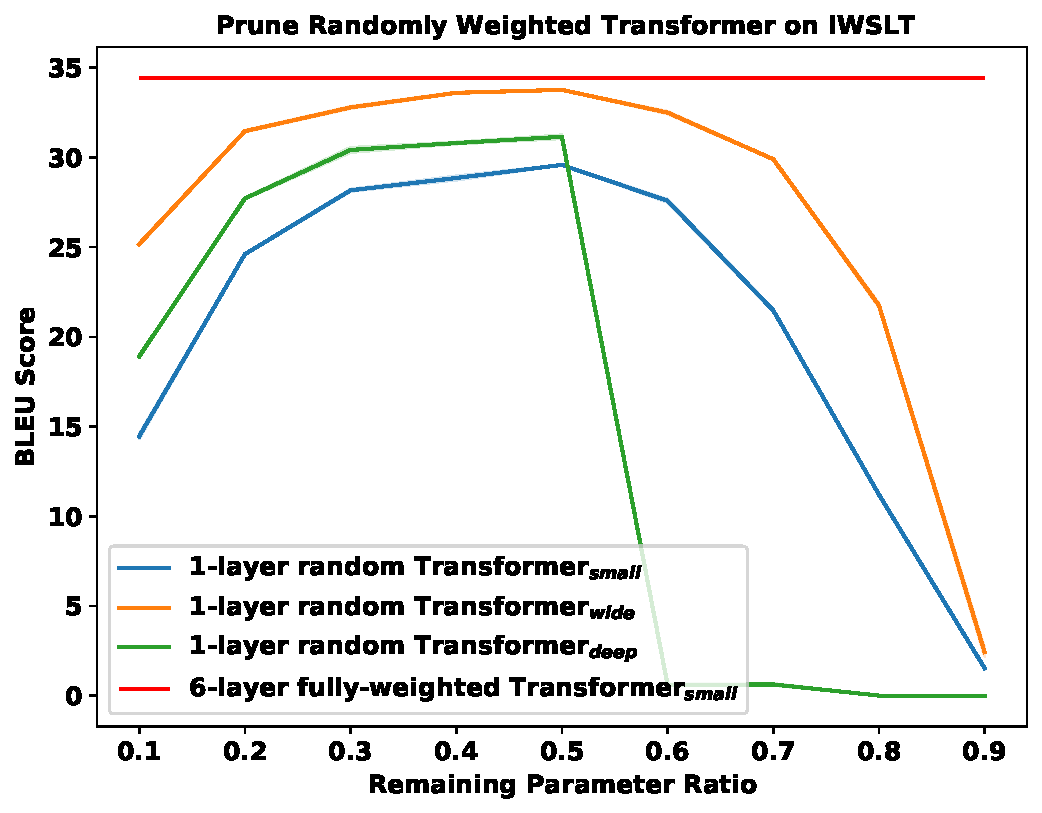
\includegraphics[width=0.8\linewidth]{fig/iwslt_widedeep.pdf}
        \vspace{-5pt}
    \caption{The effectiveness of depth and width.}
    \label{fig:res_iwslt_widedeep}
    \vspace{-10pt}
\end{figure}


\begin{figure}
    \centering
    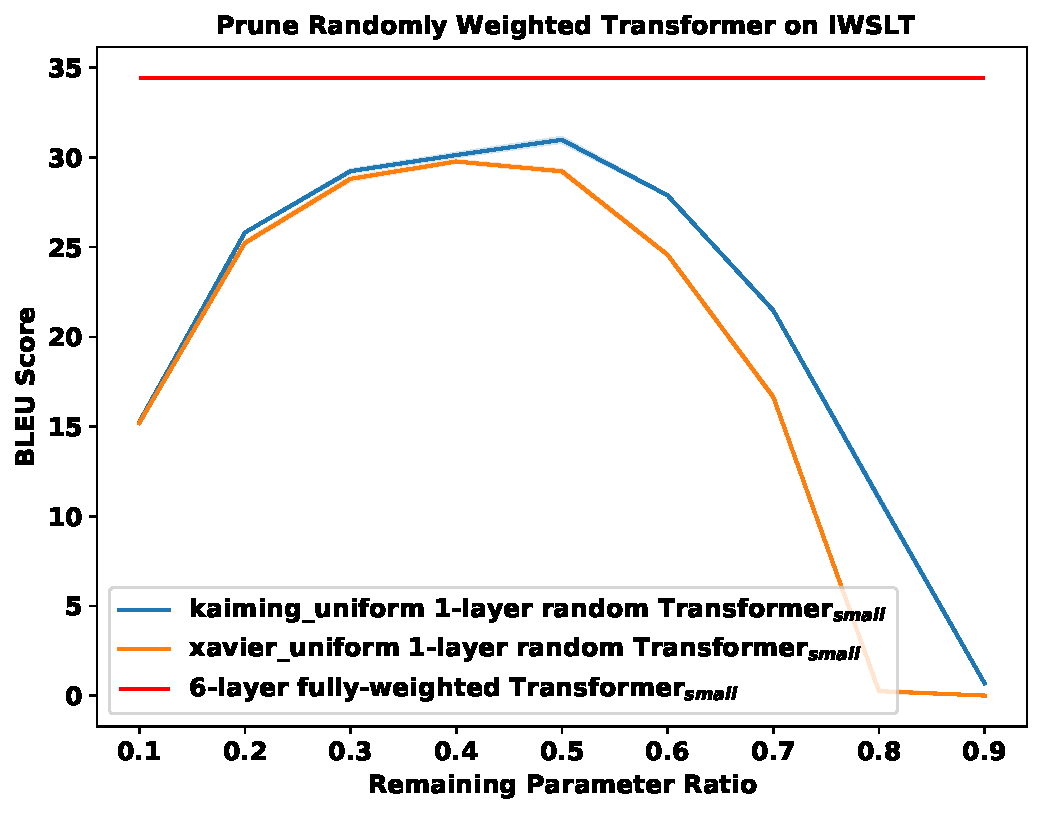
\includegraphics[width=0.8\linewidth]{fig/iwslt_init.pdf}
            \vspace{-5pt}
    \caption{The effectiveness of different initialization.}
    \label{fig:res_iwslt_init}
    \vspace{-10pt}
\end{figure}

\noindent\textbf{Different Initialization.}
Weight initialization is one of the critical components to the success of the random feature~\citep{Wieting:2019notraining,Ramanujan:2020hidden,shen2020reservoir}. 
We experiment with kaiming uniform~\citep{Ramanujan:2020hidden} and Xavier uniform~\citep{Vaswani:2017attention} initialization methods, and we scale the standard deviation by $\sqrt{1/\sigma}$ when we retain $\sigma$ randomized weights. 
As shown in~\fref{fig:res_iwslt_init}, the performance of the one-layer randomized Transformer decreases when we switch to the Xavier uniform. 
The degradation becomes larger when more randomized weights retain in the network. 





\begin{figure}
    \centering
    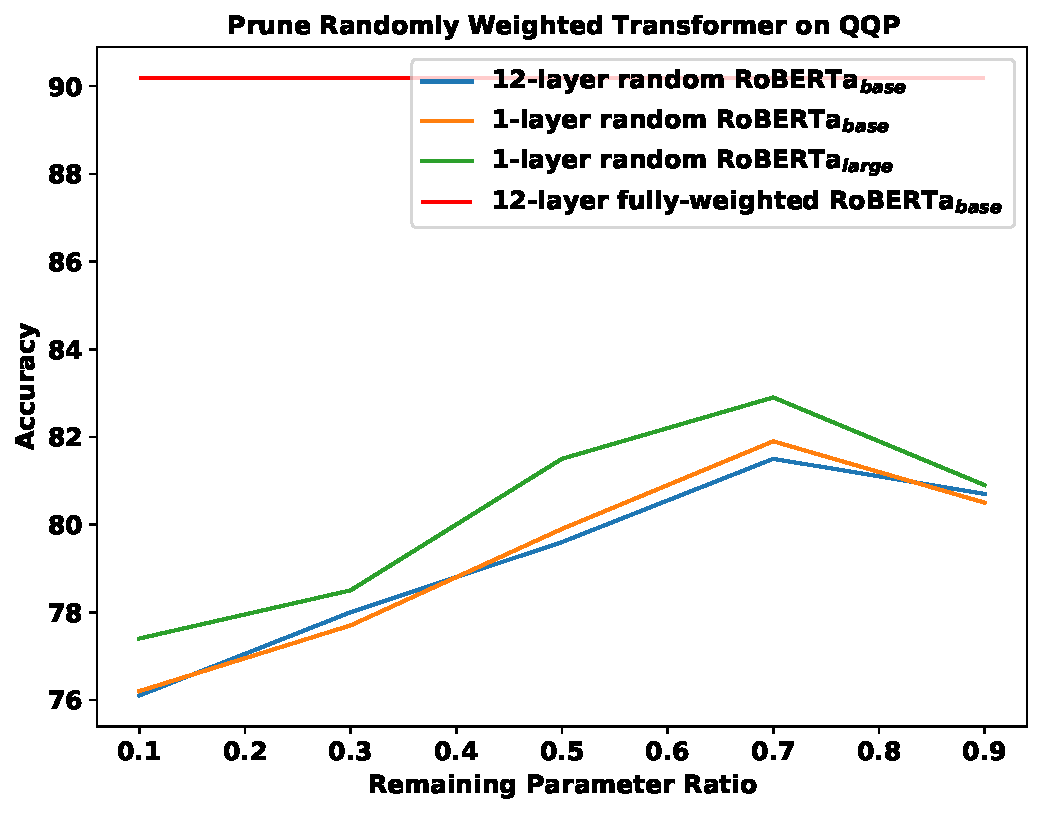
\includegraphics[width=0.8\linewidth]{fig/qqp.pdf}
    \caption{Prune Randomly Weighted Transformer performance on QQP .}
    \label{fig:qqp_base}
\end{figure}

\begin{figure}
    \centering
    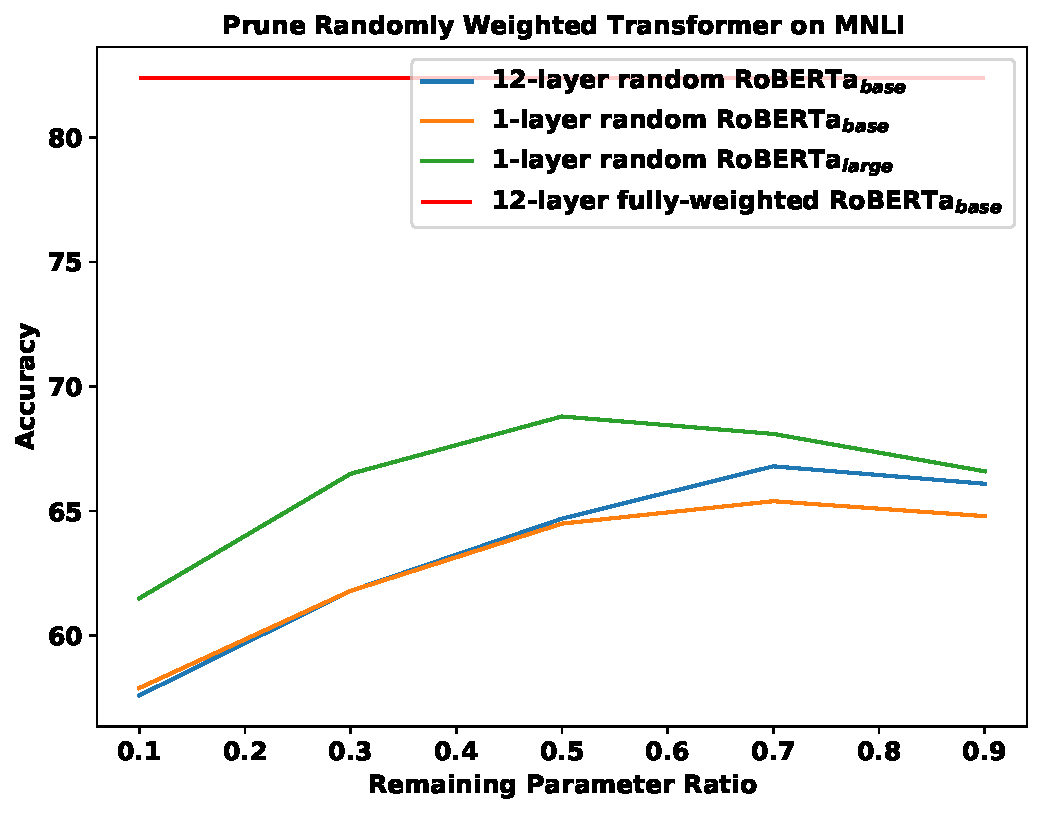
\includegraphics[width=0.8\linewidth]{fig/mnli.pdf}
    \caption{ Prune Randomly Weighted Transformer performance on MNLI.}
    \label{fig:mnli_base}
\end{figure}


\paragraph{QQP and MNLI results.} 
On QQP and MNLI, we experiment with RoBERTa$_\text{small}$ and RoBERTa$_\text{large}$, following \citet{Liu:2019roberta}. We use the pre-trained embedding layer of RoBERTa$_\text{base/large}$~\citep{Liu:2019roberta}. 
In~\fref{fig:qqp_base} and \ref{fig:mnli_base}, we show consistent results on QQP and MNLI, except that the best performing one-layer randomly weighted RoBERTa is achieved when we retain 70\% randomized weights, it reaches 79\%/91\% fully-weighted RoBERTa$_\text{base}$ accuracy on QQP and MNLI, respectively.  
The performance approaches 84\%/92\% of the aforementioned fully-weighted model performance when using the larger hidden size with one-layer randomly weighted RoBERTa$_\text{large}$. 

\paragraph{Implementation Details.} We evaluate on IWSLT14 de-en \citep{Cettolo:2015ReportOT} and WMT14 en-de \citep{bojar:2014-findings} for machine translation; QQP \citep{iyer2017qqp} and MultiNLI-matched (MNLI) \citep{Williams2017mnli} for natural language understanding.\footnote{For IWSLT, we follow the pre-processing steps in \citet{edunov:2018classical}. The train/val/test split is 129k/10k/6.8k sentences. 
For WMT, we follow pre-process as in \citet{Ott:2018scaling}, with 4.5M/16.5k/3k sentences in train/val/test.} 
We use 8 Volta V100 GPUs for WMT, and one V100 for IWSLT, QQP, and MNLI. The hyperparameters on IWSLT14 and WMT14 for training a one-layer randomized Transformer were set the same to the best-performing values from \citet{Ott:2018scaling} for training fully-weighted Transformer. The QQP and MNLI experiments followed \citet{Liu:2019roberta}. 








\newcommand{\ari}[1]{\comments{\textcolor{blue}{[\textbf{Ari:} #1]}}}
\newcommand{\ma}[1]{\textcolor{orange}{#1}}


%%%%% NEW MATH DEFINITIONS %%%%%

\usepackage{amsmath,amsfonts,bm}

% Mark sections of captions for referring to divisions of figures
\newcommand{\figleft}{{\em (Left)}}
\newcommand{\figcenter}{{\em (Center)}}
\newcommand{\figright}{{\em (Right)}}
\newcommand{\figtop}{{\em (Top)}}
\newcommand{\figbottom}{{\em (Bottom)}}
\newcommand{\captiona}{{\em (a)}}
\newcommand{\captionb}{{\em (b)}}
\newcommand{\captionc}{{\em (c)}}
\newcommand{\captiond}{{\em (d)}}

% Highlight a newly defined term
\newcommand{\newterm}[1]{{\bf #1}}


% Figure reference, lower-case.
\def\figref#1{figure~\ref{#1}}
% Figure reference, capital. For start of sentence
\def\Figref#1{Figure~\ref{#1}}
\def\twofigref#1#2{figures \ref{#1} and \ref{#2}}
\def\quadfigref#1#2#3#4{figures \ref{#1}, \ref{#2}, \ref{#3} and \ref{#4}}
% Section reference, lower-case.
\def\secref#1{section~\ref{#1}}
% Section reference, capital.
\def\Secref#1{Section~\ref{#1}}
% Reference to two sections.
\def\twosecrefs#1#2{sections \ref{#1} and \ref{#2}}
% Reference to three sections.
\def\secrefs#1#2#3{sections \ref{#1}, \ref{#2} and \ref{#3}}
% Reference to an equation, lower-case.
\def\eqref#1{equation~\ref{#1}}
% Reference to an equation, upper case
\def\Eqref#1{Equation~\ref{#1}}
% A raw reference to an equation---avoid using if possible
\def\plaineqref#1{\ref{#1}}
% Reference to a chapter, lower-case.
\def\chapref#1{chapter~\ref{#1}}
% Reference to an equation, upper case.
\def\Chapref#1{Chapter~\ref{#1}}
% Reference to a range of chapters
\def\rangechapref#1#2{chapters\ref{#1}--\ref{#2}}
% Reference to an algorithm, lower-case.
\def\algref#1{algorithm~\ref{#1}}
% Reference to an algorithm, upper case.
\def\Algref#1{Algorithm~\ref{#1}}
\def\twoalgref#1#2{algorithms \ref{#1} and \ref{#2}}
\def\Twoalgref#1#2{Algorithms \ref{#1} and \ref{#2}}
% Reference to a part, lower case
\def\partref#1{part~\ref{#1}}
% Reference to a part, upper case
\def\Partref#1{Part~\ref{#1}}
\def\twopartref#1#2{parts \ref{#1} and \ref{#2}}

\def\ceil#1{\lceil #1 \rceil}
\def\floor#1{\lfloor #1 \rfloor}
\def\1{\bm{1}}
\newcommand{\train}{\mathcal{D}}
\newcommand{\valid}{\mathcal{D_{\mathrm{valid}}}}
\newcommand{\test}{\mathcal{D_{\mathrm{test}}}}

\def\eps{{\epsilon}}


% Random variables
\def\reta{{\textnormal{$\eta$}}}
\def\ra{{\textnormal{a}}}
\def\rb{{\textnormal{b}}}
\def\rc{{\textnormal{c}}}
\def\rd{{\textnormal{d}}}
\def\re{{\textnormal{e}}}
\def\rf{{\textnormal{f}}}
\def\rg{{\textnormal{g}}}
\def\rh{{\textnormal{h}}}
\def\ri{{\textnormal{i}}}
\def\rj{{\textnormal{j}}}
\def\rk{{\textnormal{k}}}
\def\rl{{\textnormal{l}}}
% rm is already a command, just don't name any random variables m
\def\rn{{\textnormal{n}}}
\def\ro{{\textnormal{o}}}
\def\rp{{\textnormal{p}}}
\def\rq{{\textnormal{q}}}
\def\rr{{\textnormal{r}}}
\def\rs{{\textnormal{s}}}
\def\rt{{\textnormal{t}}}
\def\ru{{\textnormal{u}}}
\def\rv{{\textnormal{v}}}
\def\rw{{\textnormal{w}}}
\def\rx{{\textnormal{x}}}
\def\ry{{\textnormal{y}}}
\def\rz{{\textnormal{z}}}

% Random vectors
\def\rvepsilon{{\mathbf{\epsilon}}}
\def\rvtheta{{\mathbf{\theta}}}
\def\rva{{\mathbf{a}}}
\def\rvb{{\mathbf{b}}}
\def\rvc{{\mathbf{c}}}
\def\rvd{{\mathbf{d}}}
\def\rve{{\mathbf{e}}}
\def\rvf{{\mathbf{f}}}
\def\rvg{{\mathbf{g}}}
\def\rvh{{\mathbf{h}}}
\def\rvu{{\mathbf{i}}}
\def\rvj{{\mathbf{j}}}
\def\rvk{{\mathbf{k}}}
\def\rvl{{\mathbf{l}}}
\def\rvm{{\mathbf{m}}}
\def\rvn{{\mathbf{n}}}
\def\rvo{{\mathbf{o}}}
\def\rvp{{\mathbf{p}}}
\def\rvq{{\mathbf{q}}}
\def\rvr{{\mathbf{r}}}
\def\rvs{{\mathbf{s}}}
\def\rvt{{\mathbf{t}}}
\def\rvu{{\mathbf{u}}}
\def\rvv{{\mathbf{v}}}
\def\rvw{{\mathbf{w}}}
\def\rvx{{\mathbf{x}}}
\def\rvy{{\mathbf{y}}}
\def\rvz{{\mathbf{z}}}

% Elements of random vectors
\def\erva{{\textnormal{a}}}
\def\ervb{{\textnormal{b}}}
\def\ervc{{\textnormal{c}}}
\def\ervd{{\textnormal{d}}}
\def\erve{{\textnormal{e}}}
\def\ervf{{\textnormal{f}}}
\def\ervg{{\textnormal{g}}}
\def\ervh{{\textnormal{h}}}
\def\ervi{{\textnormal{i}}}
\def\ervj{{\textnormal{j}}}
\def\ervk{{\textnormal{k}}}
\def\ervl{{\textnormal{l}}}
\def\ervm{{\textnormal{m}}}
\def\ervn{{\textnormal{n}}}
\def\ervo{{\textnormal{o}}}
\def\ervp{{\textnormal{p}}}
\def\ervq{{\textnormal{q}}}
\def\ervr{{\textnormal{r}}}
\def\ervs{{\textnormal{s}}}
\def\ervt{{\textnormal{t}}}
\def\ervu{{\textnormal{u}}}
\def\ervv{{\textnormal{v}}}
\def\ervw{{\textnormal{w}}}
\def\ervx{{\textnormal{x}}}
\def\ervy{{\textnormal{y}}}
\def\ervz{{\textnormal{z}}}

% Random matrices
\def\rmA{{\mathbf{A}}}
\def\rmB{{\mathbf{B}}}
\def\rmC{{\mathbf{C}}}
\def\rmD{{\mathbf{D}}}
\def\rmE{{\mathbf{E}}}
\def\rmF{{\mathbf{F}}}
\def\rmG{{\mathbf{G}}}
\def\rmH{{\mathbf{H}}}
\def\rmI{{\mathbf{I}}}
\def\rmJ{{\mathbf{J}}}
\def\rmK{{\mathbf{K}}}
\def\rmL{{\mathbf{L}}}
\def\rmM{{\mathbf{M}}}
\def\rmN{{\mathbf{N}}}
\def\rmO{{\mathbf{O}}}
\def\rmP{{\mathbf{P}}}
\def\rmQ{{\mathbf{Q}}}
\def\rmR{{\mathbf{R}}}
\def\rmS{{\mathbf{S}}}
\def\rmT{{\mathbf{T}}}
\def\rmU{{\mathbf{U}}}
\def\rmV{{\mathbf{V}}}
\def\rmW{{\mathbf{W}}}
\def\rmX{{\mathbf{X}}}
\def\rmY{{\mathbf{Y}}}
\def\rmZ{{\mathbf{Z}}}

% Elements of random matrices
\def\ermA{{\textnormal{A}}}
\def\ermB{{\textnormal{B}}}
\def\ermC{{\textnormal{C}}}
\def\ermD{{\textnormal{D}}}
\def\ermE{{\textnormal{E}}}
\def\ermF{{\textnormal{F}}}
\def\ermG{{\textnormal{G}}}
\def\ermH{{\textnormal{H}}}
\def\ermI{{\textnormal{I}}}
\def\ermJ{{\textnormal{J}}}
\def\ermK{{\textnormal{K}}}
\def\ermL{{\textnormal{L}}}
\def\ermM{{\textnormal{M}}}
\def\ermN{{\textnormal{N}}}
\def\ermO{{\textnormal{O}}}
\def\ermP{{\textnormal{P}}}
\def\ermQ{{\textnormal{Q}}}
\def\ermR{{\textnormal{R}}}
\def\ermS{{\textnormal{S}}}
\def\ermT{{\textnormal{T}}}
\def\ermU{{\textnormal{U}}}
\def\ermV{{\textnormal{V}}}
\def\ermW{{\textnormal{W}}}
\def\ermX{{\textnormal{X}}}
\def\ermY{{\textnormal{Y}}}
\def\ermZ{{\textnormal{Z}}}

% Vectors
\def\vzero{{\bm{0}}}
\def\vone{{\bm{1}}}
\def\vmu{{\bm{\mu}}}
\def\vtheta{{\bm{\theta}}}
\def\va{{\bm{a}}}
\def\vb{{\bm{b}}}
\def\vc{{\bm{c}}}
\def\vd{{\bm{d}}}
\def\ve{{\bm{e}}}
\def\vf{{\bm{f}}}
\def\vg{{\bm{g}}}
\def\vh{{\bm{h}}}
\def\vi{{\bm{i}}}
\def\vj{{\bm{j}}}
\def\vk{{\bm{k}}}
\def\vl{{\bm{l}}}
\def\vm{{\bm{m}}}
\def\vn{{\bm{n}}}
\def\vo{{\bm{o}}}
\def\vp{{\bm{p}}}
\def\vq{{\bm{q}}}
\def\vr{{\bm{r}}}
\def\vs{{\bm{s}}}
\def\vt{{\bm{t}}}
\def\vu{{\bm{u}}}
\def\vv{{\bm{v}}}
\def\vw{{\bm{w}}}
\def\vx{{\bm{x}}}
\def\vy{{\bm{y}}}
\def\vz{{\bm{z}}}

% Elements of vectors
\def\evalpha{{\alpha}}
\def\evbeta{{\beta}}
\def\evepsilon{{\epsilon}}
\def\evlambda{{\lambda}}
\def\evomega{{\omega}}
\def\evmu{{\mu}}
\def\evpsi{{\psi}}
\def\evsigma{{\sigma}}
\def\evtheta{{\theta}}
\def\eva{{a}}
\def\evb{{b}}
\def\evc{{c}}
\def\evd{{d}}
\def\eve{{e}}
\def\evf{{f}}
\def\evg{{g}}
\def\evh{{h}}
\def\evi{{i}}
\def\evj{{j}}
\def\evk{{k}}
\def\evl{{l}}
\def\evm{{m}}
\def\evn{{n}}
\def\evo{{o}}
\def\evp{{p}}
\def\evq{{q}}
\def\evr{{r}}
\def\evs{{s}}
\def\evt{{t}}
\def\evu{{u}}
\def\evv{{v}}
\def\evw{{w}}
\def\evx{{x}}
\def\evy{{y}}
\def\evz{{z}}

% Matrix
\def\mA{{\bm{A}}}
\def\mB{{\bm{B}}}
\def\mC{{\bm{C}}}
\def\mD{{\bm{D}}}
\def\mE{{\bm{E}}}
\def\mF{{\bm{F}}}
\def\mG{{\bm{G}}}
\def\mH{{\bm{H}}}
\def\mI{{\bm{I}}}
\def\mJ{{\bm{J}}}
\def\mK{{\bm{K}}}
\def\mL{{\bm{L}}}
\def\mM{{\bm{M}}}
\def\mN{{\bm{N}}}
\def\mO{{\bm{O}}}
\def\mP{{\bm{P}}}
\def\mQ{{\bm{Q}}}
\def\mR{{\bm{R}}}
\def\mS{{\bm{S}}}
\def\mT{{\bm{T}}}
\def\mU{{\bm{U}}}
\def\mV{{\bm{V}}}
\def\mW{{\bm{W}}}
\def\mX{{\bm{X}}}
\def\mY{{\bm{Y}}}
\def\mZ{{\bm{Z}}}
\def\mBeta{{\bm{\beta}}}
\def\mPhi{{\bm{\Phi}}}
\def\mLambda{{\bm{\Lambda}}}
\def\mSigma{{\bm{\Sigma}}}

% Tensor
\DeclareMathAlphabet{\mathsfit}{\encodingdefault}{\sfdefault}{m}{sl}
\SetMathAlphabet{\mathsfit}{bold}{\encodingdefault}{\sfdefault}{bx}{n}
\newcommand{\tens}[1]{\bm{\mathsfit{#1}}}
\def\tA{{\tens{A}}}
\def\tB{{\tens{B}}}
\def\tC{{\tens{C}}}
\def\tD{{\tens{D}}}
\def\tE{{\tens{E}}}
\def\tF{{\tens{F}}}
\def\tG{{\tens{G}}}
\def\tH{{\tens{H}}}
\def\tI{{\tens{I}}}
\def\tJ{{\tens{J}}}
\def\tK{{\tens{K}}}
\def\tL{{\tens{L}}}
\def\tM{{\tens{M}}}
\def\tN{{\tens{N}}}
\def\tO{{\tens{O}}}
\def\tP{{\tens{P}}}
\def\tQ{{\tens{Q}}}
\def\tR{{\tens{R}}}
\def\tS{{\tens{S}}}
\def\tT{{\tens{T}}}
\def\tU{{\tens{U}}}
\def\tV{{\tens{V}}}
\def\tW{{\tens{W}}}
\def\tX{{\tens{X}}}
\def\tY{{\tens{Y}}}
\def\tZ{{\tens{Z}}}


% Graph
\def\gA{{\mathcal{A}}}
\def\gB{{\mathcal{B}}}
\def\gC{{\mathcal{C}}}
\def\gD{{\mathcal{D}}}
\def\gE{{\mathcal{E}}}
\def\gF{{\mathcal{F}}}
\def\gG{{\mathcal{G}}}
\def\gH{{\mathcal{H}}}
\def\gI{{\mathcal{I}}}
\def\gJ{{\mathcal{J}}}
\def\gK{{\mathcal{K}}}
\def\gL{{\mathcal{L}}}
\def\gM{{\mathcal{M}}}
\def\gN{{\mathcal{N}}}
\def\gO{{\mathcal{O}}}
\def\gP{{\mathcal{P}}}
\def\gQ{{\mathcal{Q}}}
\def\gR{{\mathcal{R}}}
\def\gS{{\mathcal{S}}}
\def\gT{{\mathcal{T}}}
\def\gU{{\mathcal{U}}}
\def\gV{{\mathcal{V}}}
\def\gW{{\mathcal{W}}}
\def\gX{{\mathcal{X}}}
\def\gY{{\mathcal{Y}}}
\def\gZ{{\mathcal{Z}}}

% Sets
\def\sA{{\mathbb{A}}}
\def\sB{{\mathbb{B}}}
\def\sC{{\mathbb{C}}}
\def\sD{{\mathbb{D}}}
% Don't use a set called E, because this would be the same as our symbol
% for expectation.
\def\sF{{\mathbb{F}}}
\def\sG{{\mathbb{G}}}
\def\sH{{\mathbb{H}}}
\def\sI{{\mathbb{I}}}
\def\sJ{{\mathbb{J}}}
\def\sK{{\mathbb{K}}}
\def\sL{{\mathbb{L}}}
\def\sM{{\mathbb{M}}}
\def\sN{{\mathbb{N}}}
\def\sO{{\mathbb{O}}}
\def\sP{{\mathbb{P}}}
\def\sQ{{\mathbb{Q}}}
\def\sR{{\mathbb{R}}}
\def\sS{{\mathbb{S}}}
\def\sT{{\mathbb{T}}}
\def\sU{{\mathbb{U}}}
\def\sV{{\mathbb{V}}}
\def\sW{{\mathbb{W}}}
\def\sX{{\mathbb{X}}}
\def\sY{{\mathbb{Y}}}
\def\sZ{{\mathbb{Z}}}

% Entries of a matrix
\def\emLambda{{\Lambda}}
\def\emA{{A}}
\def\emB{{B}}
\def\emC{{C}}
\def\emD{{D}}
\def\emE{{E}}
\def\emF{{F}}
\def\emG{{G}}
\def\emH{{H}}
\def\emI{{I}}
\def\emJ{{J}}
\def\emK{{K}}
\def\emL{{L}}
\def\emM{{M}}
\def\emN{{N}}
\def\emO{{O}}
\def\emP{{P}}
\def\emQ{{Q}}
\def\emR{{R}}
\def\emS{{S}}
\def\emT{{T}}
\def\emU{{U}}
\def\emV{{V}}
\def\emW{{W}}
\def\emX{{X}}
\def\emY{{Y}}
\def\emZ{{Z}}
\def\emSigma{{\Sigma}}

% entries of a tensor
% Same font as tensor, without \bm wrapper
\newcommand{\etens}[1]{\mathsfit{#1}}
\def\etLambda{{\etens{\Lambda}}}
\def\etA{{\etens{A}}}
\def\etB{{\etens{B}}}
\def\etC{{\etens{C}}}
\def\etD{{\etens{D}}}
\def\etE{{\etens{E}}}
\def\etF{{\etens{F}}}
\def\etG{{\etens{G}}}
\def\etH{{\etens{H}}}
\def\etI{{\etens{I}}}
\def\etJ{{\etens{J}}}
\def\etK{{\etens{K}}}
\def\etL{{\etens{L}}}
\def\etM{{\etens{M}}}
\def\etN{{\etens{N}}}
\def\etO{{\etens{O}}}
\def\etP{{\etens{P}}}
\def\etQ{{\etens{Q}}}
\def\etR{{\etens{R}}}
\def\etS{{\etens{S}}}
\def\etT{{\etens{T}}}
\def\etU{{\etens{U}}}
\def\etV{{\etens{V}}}
\def\etW{{\etens{W}}}
\def\etX{{\etens{X}}}
\def\etY{{\etens{Y}}}
\def\etZ{{\etens{Z}}}

% The true underlying data generating distribution
\newcommand{\pdata}{p_{\rm{data}}}
% The empirical distribution defined by the training set
\newcommand{\ptrain}{\hat{p}_{\rm{data}}}
\newcommand{\Ptrain}{\hat{P}_{\rm{data}}}
% The model distribution
\newcommand{\pmodel}{p_{\rm{model}}}
\newcommand{\Pmodel}{P_{\rm{model}}}
\newcommand{\ptildemodel}{\tilde{p}_{\rm{model}}}
% Stochastic autoencoder distributions
\newcommand{\pencode}{p_{\rm{encoder}}}
\newcommand{\pdecode}{p_{\rm{decoder}}}
\newcommand{\precons}{p_{\rm{reconstruct}}}

\newcommand{\laplace}{\mathrm{Laplace}} % Laplace distribution

\newcommand{\E}{\mathbb{E}}
\newcommand{\Ls}{\mathcal{L}}
\newcommand{\R}{\mathbb{R}}
\newcommand{\emp}{\tilde{p}}
\newcommand{\lr}{\alpha}
\newcommand{\reg}{\lambda}
\newcommand{\rect}{\mathrm{rectifier}}
\newcommand{\softmax}{\mathrm{softmax}}
\newcommand{\sigmoid}{\sigma}
\newcommand{\softplus}{\zeta}
\newcommand{\KL}{D_{\mathrm{KL}}}
\newcommand{\Var}{\mathrm{Var}}
\newcommand{\standarderror}{\mathrm{SE}}
\newcommand{\Cov}{\mathrm{Cov}}
% Wolfram Mathworld says $L^2$ is for function spaces and $\ell^2$ is for vectors
% But then they seem to use $L^2$ for vectors throughout the site, and so does
% wikipedia.
\newcommand{\normlzero}{L^0}
\newcommand{\normlone}{L^1}
\newcommand{\normltwo}{L^2}
\newcommand{\normlp}{L^p}
\newcommand{\normmax}{L^\infty}

\newcommand{\parents}{Pa} % See usage in notation.tex. Chosen to match Daphne's book.

\DeclareMathOperator*{\argmax}{arg\,max}
\DeclareMathOperator*{\argmin}{arg\,min}

\DeclareMathOperator{\sign}{sign}
\DeclareMathOperator{\Tr}{Tr}
\let\ab\allowbreak
\def\topk{\text{Top}_k\xspace}
% \usepackage{amsmath}


\newcommand\aref{Algorithm~\ref}
\newcommand\appref{Appendix~\ref}
\newcommand\eref{Eq.~\ref}
\newcommand\fref{Fig.~\ref}
\newcommand\tref{Tab.~\ref}
\newcommand\sref{\textsection~\ref}
\begin{abstract}
We demonstrate that, hidden within one-layer randomly weighted neural networks, there exist subnetworks that can achieve impressive performance, without ever modifying the weight initializations, on machine translation tasks. 
To find subnetworks for one-layer randomly weighted neural networks, we apply different binary masks to the same weight matrix to generate different layers. 
Hidden within a one-layer randomly weighted Transformer, we find that subnetworks that can achieve 29.45/17.29 BLEU on IWSLT14/WMT14. 
Using a fixed pre-trained embedding layer, the previously found subnetworks are smaller than, but can match 98\%/92\% (34.14/25.24 BLEU) of the performance of, a trained Transformer$_\text{small/base}$ on IWSLT14/WMT14. 
Furthermore, we demonstrate the effectiveness of larger and deeper transformers in this setting, as well as the impact of different initialization methods.\footnote{We released the source code at \url{https://github.com/sIncerass/one_layer_lottery_ticket}.}
\end{abstract}
% This must be in the first 5 lines to tell arXiv to use pdfLaTeX, which is strongly recommended.
\pdfoutput=1
% In particular, the hyperref package requires pdfLaTeX in order to break URLs across lines.

\documentclass[11pt]{article}

% Remove the "review" option to generate the final version.
% \usepackage[review]{emnlp2021}

\usepackage[final]{emnlp2021}
\usepackage{times}
\usepackage{latexsym}

% Optional math commands from https://github.com/goodfeli/dlbook_notation.
\newcommand{\Brittany}[1]{[\textbf{Brittany}:~{\color{purple} #1}]}
\newcommand{\Markus}[1]{[\textbf{Markus}:{\color{magenta} #1}]}
\newcommand{\Christoph}[1]{[\textbf{Christoph}:~{\color{blue} #1}]}

\newcommand{\ts}{TypeScript}
\newcommand{\js}{JavaScript}

%research questions
\newcommand{\rqone}{What errors does \ts\ detect in NPM documentation?}
\newcommand{\rqtwo}{How does error detection differ between ESLint and \ts?}
\newcommand{\rqthree}{What is the impact of NCC on the set of NPM snippets?}
\newcommand{\rqfour}{How does NCC compare to NCQ's code corrections?}
\newcommand{\rqfive}{How does NCC compare to manual fixes?}

%hyperref setup
\hypersetup{
    colorlinks=true,
    linkcolor=blue,
    anchorcolor=blue,
    filecolor=blue,      
    citecolor=blue,
    urlcolor=blue
}

%define colours
\definecolor{lightgreen}{rgb}{0.8,1,0.8}
\definecolor{lightyellow}{rgb}{1,1,0.8}
\definecolor{lightred}{rgb}{1,0.8,0.8}
\definecolor{baseColour}{RGB}{255, 128, 85}
\definecolor{ncqColour}{RGB}{118, 165, 175}
\definecolor{ncqColour2}{RGB}{162, 196, 201}

%algorithm comment style
\newcommand\mycommfont[1]{\footnotesize\ttfamily\textcolor{blue}{#1}}
\SetCommentSty{mycommfont}
%alg options
\SetAlFnt{\small}
\SetAlCapFnt{\small}
\SetAlCapNameFnt{\small}
\algsetup{linenosize=\tiny}

%lsting setup
\lstdefinelanguage{javascript}{
    keywords={typeof, new, true, false, catch, function, return, null, catch, switch, var, if, in, while, do, else, case, break},
    keywordstyle=\bfseries,
    ndkeywords={class, export, boolean, throw, implements, import, this},
    ndkeywordstyle=\color{darkgray}\bfseries,
    identifierstyle=\color{black},
    sensitive=false,
    comment=[l]{//},
    morecomment=[s]{/*}{*/},
    commentstyle=\color{blue}\ttfamily,
    stringstyle=\color{purple}\ttfamily,
    morestring=[b]',
    morestring=[b]"
}
\newcommand{\lstbg}[3][0pt]{{\fboxsep#1\colorbox{#2}{\strut #3}}}
\lstdefinelanguage{diff}{
    morecomment=[f][\lstbg{lightgreen}]+,
    morecomment=[f][\lstbg{lightred}]-,
    morecomment=[f][\lstbg{lightyellow}]\\,
    keywords={typeof, new, true, false, catch, function, return, null, catch, switch, var, if, in, while, do, else, case, break},
    keywordstyle=\bfseries,
    ndkeywords={class, export, boolean, throw, implements, import, this},
    ndkeywordstyle=\color{darkgray}\bfseries,
    identifierstyle=\color{black},
    sensitive=false,
    morecomment=[s]{/*}{*/},
    commentstyle=\color{blue}\ttfamily,
    stringstyle=\color{purple}\ttfamily,
    morestring=[b]',
    morestring=[b]"
}
\lstset{
    frame = single,
    tabsize=1,
    showstringspaces=false,
    language=javascript,
    basicstyle=\fontsize{7}{6}\selectfont\ttfamily,
    breaklines=true, 
    breakatwhitespace=false,   % sets if automatic breaks should only happen at
    numbers=left, 
    firstnumber=1,
    numberstyle=\tiny, 
    stepnumber=1, 
    numbersep=5pt,
    float,
    aboveskip=0pt,
    belowskip=0pt,
    xleftmargin=.02\textwidth,
    xrightmargin=.02\textwidth,
    escapeinside={\%*}{*)},          % if you want to add LaTeX within  % your code 
}

\addto\extrasenglish{%
  \def\chapterautorefname{Chapter}%
  \def\sectionautorefname{Section}%
  \def\algorithmautorefname{Algorithm}%
  \def\subsectionautorefname{Section}%
  \def\subsubsectionautorefname{Section}%
}

%tikz
\usetikzlibrary{
    arrows.meta,
    chains,
    scopes,
    positioning,
    shapes.geometric
}
% layers
\pgfdeclarelayer{background}
\pgfdeclarelayer{foreground}
\pgfsetlayers{background,main,foreground}

% styles     
\tikzset{
    processDiagram/.style={
        startstop/.style={
            rectangle,
            draw,
            minimum width=3cm, 
            minimum height=0.8cm,
            join = by arrow,
            fill = black!0,
        },
        decision/.style = {
            diamond,
            aspect=1.7,
            draw,
            minimum width=2.5cm, 
            minimum height=1cm, 
            align=center,
            join = by arrow,
            fill = black!0,
        },
        process/.style = {
            rectangle, 
            rounded corners, 
            draw,
            minimum width=3cm,
            minimum height=0.8cm, 
            align=center,
            join = by arrow,
            fill = black!0,
        },
        process2/.style = {
            rectangle, 
            rounded corners, 
            draw,
            minimum width=3cm,
            minimum height=0.8cm, 
            align=center,
            join = by arrow,
            fill = ncqColour2,
        },
        line/.style = {
            -
        },
        invisible/.style = {
            join = by line,
            minimum width=0cm, 
            minimum height=0cm,
            inner sep=0pt,
        },
        invisititle/.style ={
            font = \bfseries,
            join = by arrow,
            outer sep = 5pt,
        },
        title/.style = {
            font = \bfseries,
            fill = black!20,
            join = by arrow,
            minimum width = 3cm,
            minimum height=0.8cm,
            draw,
        },
        output/.style ={
            join = by line,
            minimum width=0cm, 
            minimum height=0cm,
            inner sep=0pt,
            font = \itshape,
            align = center,
        },
        arrow/.style = {
            ->
        },
    }
}

\usepackage{hyperref}
\usepackage{url}
\usepackage{graphicx,subcaption}
\usepackage{booktabs}
\usepackage{multirow}
\newcommand\setrow[1]{\gdef\currentrowstyle{#1}%
    #1\ignorespaces
}


\newcommand{\textapprox}{\raisebox{0.5ex}{\texttildelow}}


% -------------- Our Packages and Commands ----------------

\newcommand{\sheng}[1]{\textcolor{magenta}{sheng:\ #1}}
\newcommand{\douwe}[1]{\textcolor{blue}{Douwe:\ #1}}
\newcommand{\zhewei}[1]{\textcolor{orange}{Zhewei:\ #1}}
\newcommand\blfootnote[1]{%
  \begingroup
  \renewcommand\thefootnote{}\footnote{#1}%
  \addtocounter{footnote}{-1}%
  \endgroup
}

% \def\baselinestretch{0.985}

\title{What’s Hidden in a One-layer Randomly Weighted Transformer?}

\author{
Sheng Shen$^{\dagger*}$, Zhewei Yao$^{\dagger*}$,  Douwe Kiela$^\ddagger$, Kurt Keutzer$^\dagger$ and Michael W. Mahoney$^\dagger$\\
 $^\dagger$UC Berkeley; $^\ddagger$Facebook AI Research\\
 \texttt{\{sheng.s,zheweiy\}@berkeley.edu, dkiela@fb.com}
}

\begin{document}
\maketitle

%%%%%%%% BODY TEXT
\input _s0_abstract.tex
\blfootnote{$^*$Equal contribution.}
% \vspace{-4mm}
\input _s1_intro.tex
% \vspace{-4mm}
\input _s2_related_work.tex
\input _s3_method.tex
% \vspace{-4mm}
\input _s4_results.tex
% \vspace{-4mm}
\input _s5_conclusion.tex
% \vspace{-4mm}

% \clearpage
\bibliography{ref}
\bibliographystyle{acl_natbib}

\clearpage


\end{document}

% This must be in the first 5 lines to tell arXiv to use pdfLaTeX, which is strongly recommended.
\pdfoutput=1
% In particular, the hyperref package requires pdfLaTeX in order to break URLs across lines.

\documentclass[11pt]{article}

% Remove the "review" option to generate the final version.
% \usepackage[review]{emnlp2021}

\usepackage[review]{emnlp2021}
\usepackage{times}
\usepackage{latexsym}

% Optional math commands from https://github.com/goodfeli/dlbook_notation.
\newcommand{\Brittany}[1]{[\textbf{Brittany}:~{\color{purple} #1}]}
\newcommand{\Markus}[1]{[\textbf{Markus}:{\color{magenta} #1}]}
\newcommand{\Christoph}[1]{[\textbf{Christoph}:~{\color{blue} #1}]}

\newcommand{\ts}{TypeScript}
\newcommand{\js}{JavaScript}

%research questions
\newcommand{\rqone}{What errors does \ts\ detect in NPM documentation?}
\newcommand{\rqtwo}{How does error detection differ between ESLint and \ts?}
\newcommand{\rqthree}{What is the impact of NCC on the set of NPM snippets?}
\newcommand{\rqfour}{How does NCC compare to NCQ's code corrections?}
\newcommand{\rqfive}{How does NCC compare to manual fixes?}

%hyperref setup
\hypersetup{
    colorlinks=true,
    linkcolor=blue,
    anchorcolor=blue,
    filecolor=blue,      
    citecolor=blue,
    urlcolor=blue
}

%define colours
\definecolor{lightgreen}{rgb}{0.8,1,0.8}
\definecolor{lightyellow}{rgb}{1,1,0.8}
\definecolor{lightred}{rgb}{1,0.8,0.8}
\definecolor{baseColour}{RGB}{255, 128, 85}
\definecolor{ncqColour}{RGB}{118, 165, 175}
\definecolor{ncqColour2}{RGB}{162, 196, 201}

%algorithm comment style
\newcommand\mycommfont[1]{\footnotesize\ttfamily\textcolor{blue}{#1}}
\SetCommentSty{mycommfont}
%alg options
\SetAlFnt{\small}
\SetAlCapFnt{\small}
\SetAlCapNameFnt{\small}
\algsetup{linenosize=\tiny}

%lsting setup
\lstdefinelanguage{javascript}{
    keywords={typeof, new, true, false, catch, function, return, null, catch, switch, var, if, in, while, do, else, case, break},
    keywordstyle=\bfseries,
    ndkeywords={class, export, boolean, throw, implements, import, this},
    ndkeywordstyle=\color{darkgray}\bfseries,
    identifierstyle=\color{black},
    sensitive=false,
    comment=[l]{//},
    morecomment=[s]{/*}{*/},
    commentstyle=\color{blue}\ttfamily,
    stringstyle=\color{purple}\ttfamily,
    morestring=[b]',
    morestring=[b]"
}
\newcommand{\lstbg}[3][0pt]{{\fboxsep#1\colorbox{#2}{\strut #3}}}
\lstdefinelanguage{diff}{
    morecomment=[f][\lstbg{lightgreen}]+,
    morecomment=[f][\lstbg{lightred}]-,
    morecomment=[f][\lstbg{lightyellow}]\\,
    keywords={typeof, new, true, false, catch, function, return, null, catch, switch, var, if, in, while, do, else, case, break},
    keywordstyle=\bfseries,
    ndkeywords={class, export, boolean, throw, implements, import, this},
    ndkeywordstyle=\color{darkgray}\bfseries,
    identifierstyle=\color{black},
    sensitive=false,
    morecomment=[s]{/*}{*/},
    commentstyle=\color{blue}\ttfamily,
    stringstyle=\color{purple}\ttfamily,
    morestring=[b]',
    morestring=[b]"
}
\lstset{
    frame = single,
    tabsize=1,
    showstringspaces=false,
    language=javascript,
    basicstyle=\fontsize{7}{6}\selectfont\ttfamily,
    breaklines=true, 
    breakatwhitespace=false,   % sets if automatic breaks should only happen at
    numbers=left, 
    firstnumber=1,
    numberstyle=\tiny, 
    stepnumber=1, 
    numbersep=5pt,
    float,
    aboveskip=0pt,
    belowskip=0pt,
    xleftmargin=.02\textwidth,
    xrightmargin=.02\textwidth,
    escapeinside={\%*}{*)},          % if you want to add LaTeX within  % your code 
}

\addto\extrasenglish{%
  \def\chapterautorefname{Chapter}%
  \def\sectionautorefname{Section}%
  \def\algorithmautorefname{Algorithm}%
  \def\subsectionautorefname{Section}%
  \def\subsubsectionautorefname{Section}%
}

%tikz
\usetikzlibrary{
    arrows.meta,
    chains,
    scopes,
    positioning,
    shapes.geometric
}
% layers
\pgfdeclarelayer{background}
\pgfdeclarelayer{foreground}
\pgfsetlayers{background,main,foreground}

% styles     
\tikzset{
    processDiagram/.style={
        startstop/.style={
            rectangle,
            draw,
            minimum width=3cm, 
            minimum height=0.8cm,
            join = by arrow,
            fill = black!0,
        },
        decision/.style = {
            diamond,
            aspect=1.7,
            draw,
            minimum width=2.5cm, 
            minimum height=1cm, 
            align=center,
            join = by arrow,
            fill = black!0,
        },
        process/.style = {
            rectangle, 
            rounded corners, 
            draw,
            minimum width=3cm,
            minimum height=0.8cm, 
            align=center,
            join = by arrow,
            fill = black!0,
        },
        process2/.style = {
            rectangle, 
            rounded corners, 
            draw,
            minimum width=3cm,
            minimum height=0.8cm, 
            align=center,
            join = by arrow,
            fill = ncqColour2,
        },
        line/.style = {
            -
        },
        invisible/.style = {
            join = by line,
            minimum width=0cm, 
            minimum height=0cm,
            inner sep=0pt,
        },
        invisititle/.style ={
            font = \bfseries,
            join = by arrow,
            outer sep = 5pt,
        },
        title/.style = {
            font = \bfseries,
            fill = black!20,
            join = by arrow,
            minimum width = 3cm,
            minimum height=0.8cm,
            draw,
        },
        output/.style ={
            join = by line,
            minimum width=0cm, 
            minimum height=0cm,
            inner sep=0pt,
            font = \itshape,
            align = center,
        },
        arrow/.style = {
            ->
        },
    }
}

\usepackage{hyperref}
\usepackage{url}
\usepackage{graphicx,subcaption}
\usepackage{booktabs}
\usepackage{multirow}
\newcommand\setrow[1]{\gdef\currentrowstyle{#1}%
    #1\ignorespaces
}


\newcommand{\textapprox}{\raisebox{0.5ex}{\texttildelow}}


% -------------- Our Packages and Commands ----------------

\newcommand{\sheng}[1]{\textcolor{magenta}{sheng:\ #1}}
\newcommand{\douwe}[1]{\textcolor{blue}{Douwe:\ #1}}
\newcommand{\zhewei}[1]{\textcolor{orange}{Zhewei:\ #1}}

% \def\baselinestretch{0.985}

\title{Supplementary Materials for \\
What’s Hidden in a One-layer Randomly Weighted Transformer?}

\author{
None
}


\begin{document}
\maketitle

% %%%%%%%% BODY TEXT
% \input _s0_abstract.tex
% % \vspace{-4mm}
% \input _s1_intro.tex
% % \vspace{-4mm}
% \input _s2_related_work.tex
% \input _s3_method.tex
% % \vspace{-4mm}
% \input _s4_results.tex
% % \vspace{-4mm}
% \input _s5_discussion.tex
% % \vspace{-4mm}
% \input _s6_conclusion.tex
% % \vspace{-4mm}


\input _s7_appendix.tex
% \clearpage
\bibliography{ref}
\bibliographystyle{acl_natbib}

\clearpage



\end{document}

% This must be in the first 5 lines to tell arXiv to use pdfLaTeX, which is strongly recommended.
\pdfoutput=1
% In particular, the hyperref package requires pdfLaTeX in order to break URLs across lines.

\documentclass[11pt]{article}

% Remove the "review" option to generate the final version.
% \usepackage[review]{emnlp2021}

\usepackage[review]{emnlp2021}
\usepackage{times}
\usepackage{latexsym}

% Optional math commands from https://github.com/goodfeli/dlbook_notation.
\newcommand{\Brittany}[1]{[\textbf{Brittany}:~{\color{purple} #1}]}
\newcommand{\Markus}[1]{[\textbf{Markus}:{\color{magenta} #1}]}
\newcommand{\Christoph}[1]{[\textbf{Christoph}:~{\color{blue} #1}]}

\newcommand{\ts}{TypeScript}
\newcommand{\js}{JavaScript}

%research questions
\newcommand{\rqone}{What errors does \ts\ detect in NPM documentation?}
\newcommand{\rqtwo}{How does error detection differ between ESLint and \ts?}
\newcommand{\rqthree}{What is the impact of NCC on the set of NPM snippets?}
\newcommand{\rqfour}{How does NCC compare to NCQ's code corrections?}
\newcommand{\rqfive}{How does NCC compare to manual fixes?}

%hyperref setup
\hypersetup{
    colorlinks=true,
    linkcolor=blue,
    anchorcolor=blue,
    filecolor=blue,      
    citecolor=blue,
    urlcolor=blue
}

%define colours
\definecolor{lightgreen}{rgb}{0.8,1,0.8}
\definecolor{lightyellow}{rgb}{1,1,0.8}
\definecolor{lightred}{rgb}{1,0.8,0.8}
\definecolor{baseColour}{RGB}{255, 128, 85}
\definecolor{ncqColour}{RGB}{118, 165, 175}
\definecolor{ncqColour2}{RGB}{162, 196, 201}

%algorithm comment style
\newcommand\mycommfont[1]{\footnotesize\ttfamily\textcolor{blue}{#1}}
\SetCommentSty{mycommfont}
%alg options
\SetAlFnt{\small}
\SetAlCapFnt{\small}
\SetAlCapNameFnt{\small}
\algsetup{linenosize=\tiny}

%lsting setup
\lstdefinelanguage{javascript}{
    keywords={typeof, new, true, false, catch, function, return, null, catch, switch, var, if, in, while, do, else, case, break},
    keywordstyle=\bfseries,
    ndkeywords={class, export, boolean, throw, implements, import, this},
    ndkeywordstyle=\color{darkgray}\bfseries,
    identifierstyle=\color{black},
    sensitive=false,
    comment=[l]{//},
    morecomment=[s]{/*}{*/},
    commentstyle=\color{blue}\ttfamily,
    stringstyle=\color{purple}\ttfamily,
    morestring=[b]',
    morestring=[b]"
}
\newcommand{\lstbg}[3][0pt]{{\fboxsep#1\colorbox{#2}{\strut #3}}}
\lstdefinelanguage{diff}{
    morecomment=[f][\lstbg{lightgreen}]+,
    morecomment=[f][\lstbg{lightred}]-,
    morecomment=[f][\lstbg{lightyellow}]\\,
    keywords={typeof, new, true, false, catch, function, return, null, catch, switch, var, if, in, while, do, else, case, break},
    keywordstyle=\bfseries,
    ndkeywords={class, export, boolean, throw, implements, import, this},
    ndkeywordstyle=\color{darkgray}\bfseries,
    identifierstyle=\color{black},
    sensitive=false,
    morecomment=[s]{/*}{*/},
    commentstyle=\color{blue}\ttfamily,
    stringstyle=\color{purple}\ttfamily,
    morestring=[b]',
    morestring=[b]"
}
\lstset{
    frame = single,
    tabsize=1,
    showstringspaces=false,
    language=javascript,
    basicstyle=\fontsize{7}{6}\selectfont\ttfamily,
    breaklines=true, 
    breakatwhitespace=false,   % sets if automatic breaks should only happen at
    numbers=left, 
    firstnumber=1,
    numberstyle=\tiny, 
    stepnumber=1, 
    numbersep=5pt,
    float,
    aboveskip=0pt,
    belowskip=0pt,
    xleftmargin=.02\textwidth,
    xrightmargin=.02\textwidth,
    escapeinside={\%*}{*)},          % if you want to add LaTeX within  % your code 
}

\addto\extrasenglish{%
  \def\chapterautorefname{Chapter}%
  \def\sectionautorefname{Section}%
  \def\algorithmautorefname{Algorithm}%
  \def\subsectionautorefname{Section}%
  \def\subsubsectionautorefname{Section}%
}

%tikz
\usetikzlibrary{
    arrows.meta,
    chains,
    scopes,
    positioning,
    shapes.geometric
}
% layers
\pgfdeclarelayer{background}
\pgfdeclarelayer{foreground}
\pgfsetlayers{background,main,foreground}

% styles     
\tikzset{
    processDiagram/.style={
        startstop/.style={
            rectangle,
            draw,
            minimum width=3cm, 
            minimum height=0.8cm,
            join = by arrow,
            fill = black!0,
        },
        decision/.style = {
            diamond,
            aspect=1.7,
            draw,
            minimum width=2.5cm, 
            minimum height=1cm, 
            align=center,
            join = by arrow,
            fill = black!0,
        },
        process/.style = {
            rectangle, 
            rounded corners, 
            draw,
            minimum width=3cm,
            minimum height=0.8cm, 
            align=center,
            join = by arrow,
            fill = black!0,
        },
        process2/.style = {
            rectangle, 
            rounded corners, 
            draw,
            minimum width=3cm,
            minimum height=0.8cm, 
            align=center,
            join = by arrow,
            fill = ncqColour2,
        },
        line/.style = {
            -
        },
        invisible/.style = {
            join = by line,
            minimum width=0cm, 
            minimum height=0cm,
            inner sep=0pt,
        },
        invisititle/.style ={
            font = \bfseries,
            join = by arrow,
            outer sep = 5pt,
        },
        title/.style = {
            font = \bfseries,
            fill = black!20,
            join = by arrow,
            minimum width = 3cm,
            minimum height=0.8cm,
            draw,
        },
        output/.style ={
            join = by line,
            minimum width=0cm, 
            minimum height=0cm,
            inner sep=0pt,
            font = \itshape,
            align = center,
        },
        arrow/.style = {
            ->
        },
    }
}

\usepackage{hyperref}
\usepackage{url}
\usepackage{graphicx,subcaption}
\usepackage{booktabs}
\usepackage{multirow}
\newcommand\setrow[1]{\gdef\currentrowstyle{#1}%
    #1\ignorespaces
}


\newcommand{\textapprox}{\raisebox{0.5ex}{\texttildelow}}


% -------------- Our Packages and Commands ----------------

\newcommand{\sheng}[1]{\textcolor{magenta}{sheng:\ #1}}
\newcommand{\douwe}[1]{\textcolor{blue}{Douwe:\ #1}}
\newcommand{\zhewei}[1]{\textcolor{orange}{Zhewei:\ #1}}

% \def\baselinestretch{0.985}

\title{Appendix: What’s Hidden in a One-layer Randomly Weighted Transformer?}

\author{
None
}


\begin{document}
\maketitle

%%%%%%%% BODY TEXT
\input _s7_appendix.tex


% \clearpage
\bibliography{ref}
\bibliographystyle{acl_natbib}






\end{document}

\vspace{-2mm}
\section{Methodology}
\label{sec:methodology}
\vspace{-1mm}

\noindent\textbf{Finding a Supermask for Randomly Weighted Transformer.} 
In a general pruning framework, denote weight matrix as $\rmW\in\sR^{d\times d}$  ($\rmW$ could be a non-square matrix), input as $x\in\sR^d$ and the network as $f(x; \rmW)$. 
A subnetwork defined is $f(x; \rmW \odot \rmM)$, where $\rmM\in\sR^{d\times d}$ is a binary matrix and $\odot$ is the element-wise product. 
To find the subnetwork for a randomly weighted network, $\rmM\in\sR^{d\times d}$ is trained while $\rmW$ is kept at a random initialization. 
Following~\citet{Ramanujan:2020hidden}, denote $\rmS\in\sR^{d\times d}$ as the associated importance score matrix of $\rmW$, which is learnable during training. 
We keep top-k percents of weights by the importance score of $\rmS$ to compute $\rmM$, i.e., 
\begin{equation*}
\label{eq:topk}
\resizebox{\linewidth}{!}{$\displaystyle
% \small
\rmM = \text{Top}_k(\rmS), \text{where}
    ~\text{Top}_k(\rmS_{i, j}) = 
    \begin{cases}
    ~1 &\rmS_{i, j}\text{ in top k\%},\\
    ~0 &\text{else}.
    \end{cases}
    $
}
\end{equation*}
Note that $\text{Top}_k$ is an undifferentiated function.
To enable training of $\rmS$, we use the straight-through gradient estimator \citep{bengio2013estimating}, in which $\text{Top}_k$ is treated as the identity in backpropagation. 
During inference, we can simply construct and store the binary Supermask $\rmM$ and the floating-point $\rmW$ while dropping $\rmS$ for future usage. 

\noindent\textbf{One-layer randomly weighted Transformer.}
We use the Transformer architecture (see ~\newcite{Vaswani:2017attention} for more details).
For a general randomly weighted Transformer model with Supermask, there exist $\rmM_l$s and $\rmW_l$s for all layers $l \in \{1, ... L\}$. 
Due to the natural property of layer stacking in Transformers, all $\rmW_l$s have the same shape with the same initialization method. 
This leads to an unexplored question: ``What's hidden in a one-layer (instead of L-layer) randomly weighted transformer?''



\begin{figure*}
    \centering
    \begin{subfigure}{.4\textwidth}
        \centering
        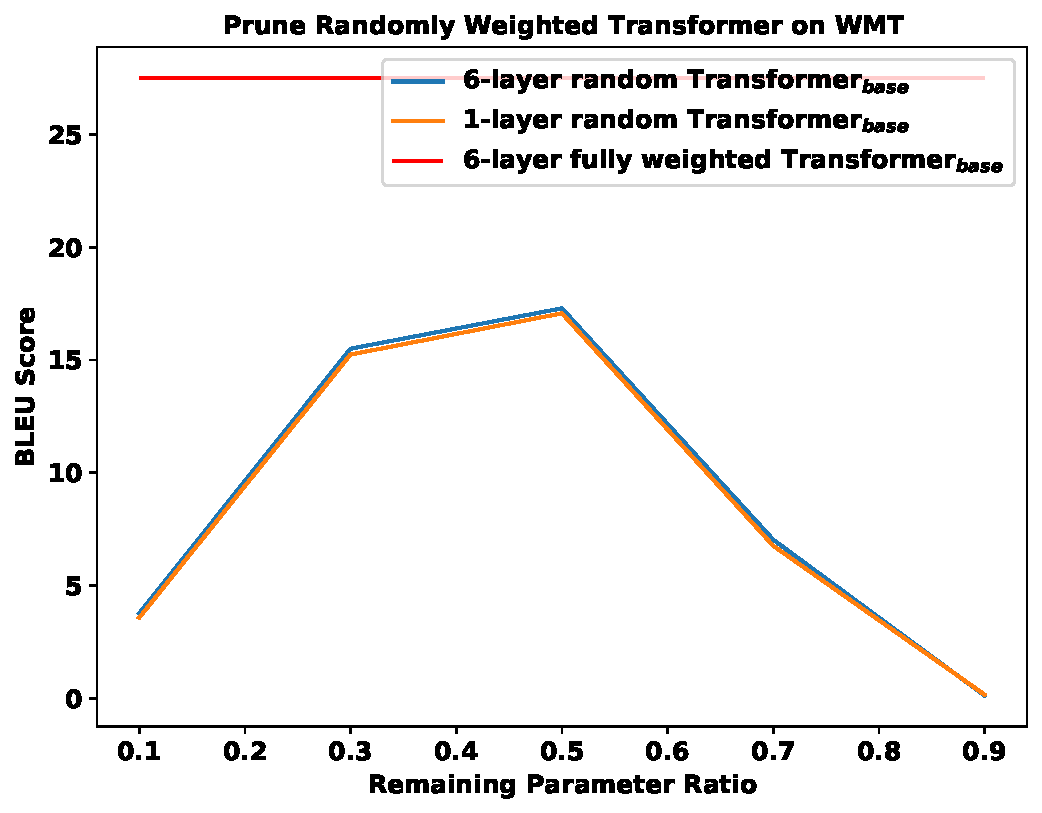
\includegraphics[width=\textwidth]{fig/wmt_result.pdf}
    \end{subfigure}%
    \begin{subfigure}{.4\textwidth}
        \centering
        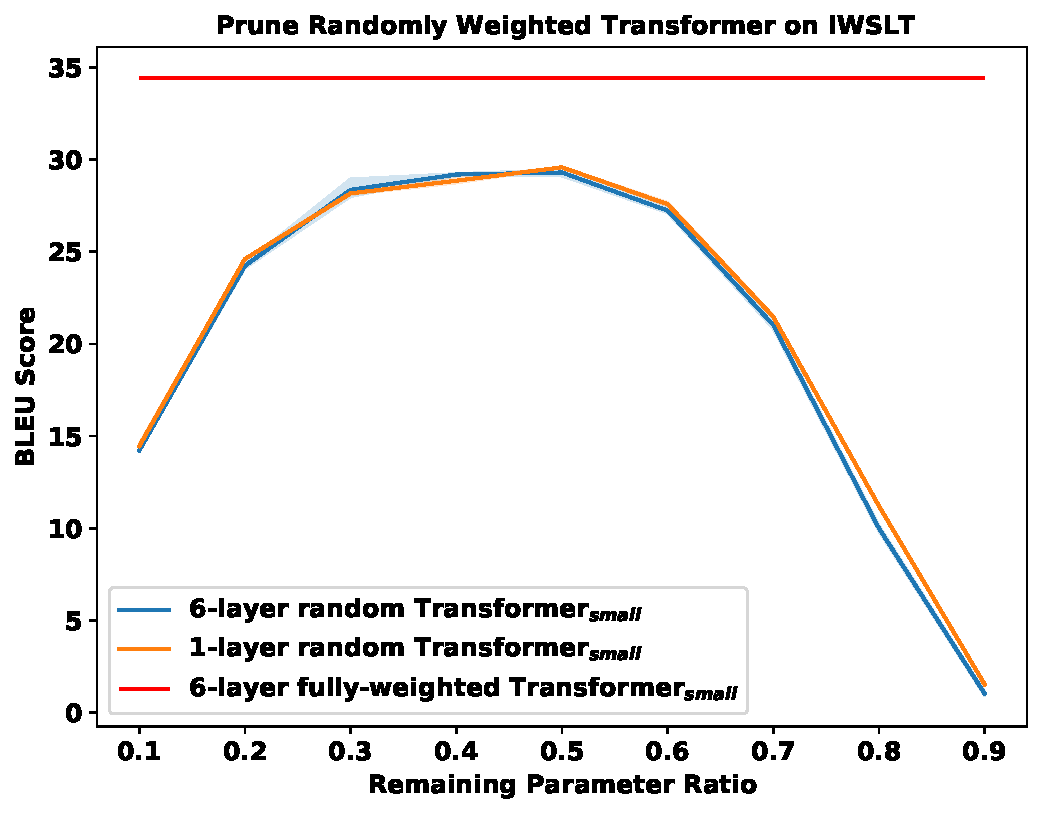
\includegraphics[width=\textwidth]{fig/iwslt_base.pdf}
    \end{subfigure}
            \vspace{-5pt}
    \caption{Prune Randomly Weighted Transformer performance on WMT14 (left) and IWSLT14 (right).}
    \label{fig:mt_base}
            \vspace{-5pt}
\end{figure*}

\begin{figure*}
    \centering
    \begin{subfigure}{.4\textwidth}
        \centering
        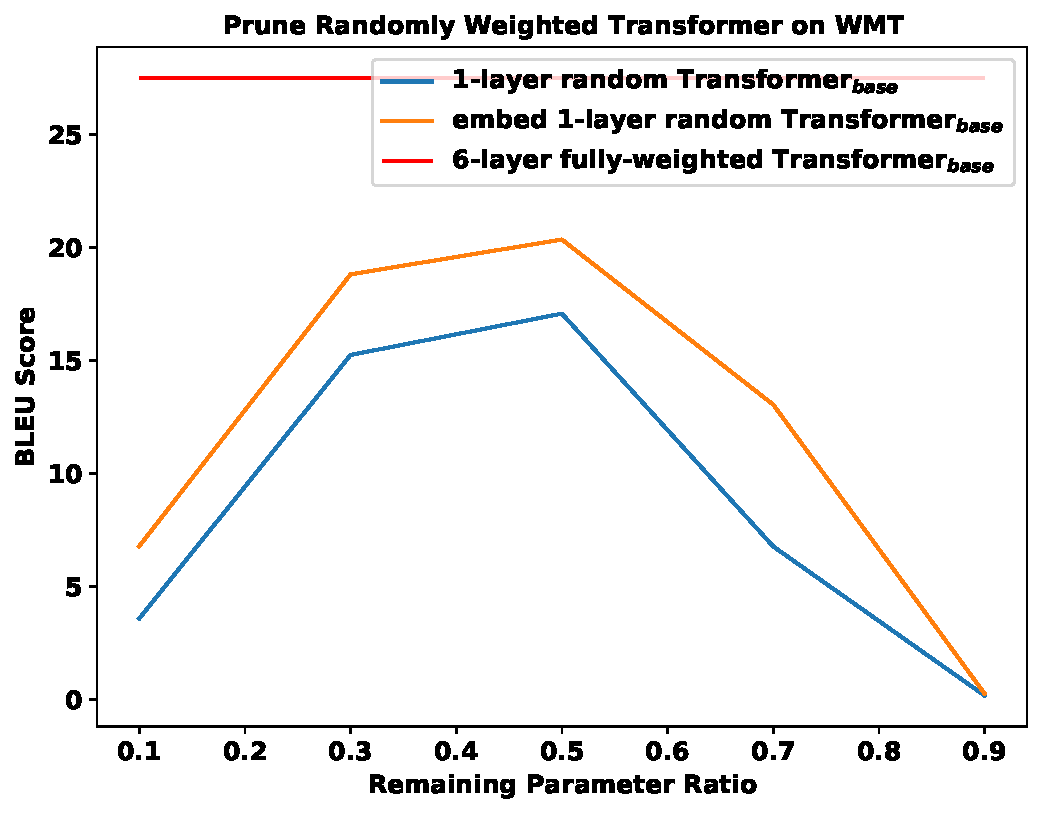
\includegraphics[width=\textwidth]{fig/wmt_embed.pdf}
    \end{subfigure}%
    \begin{subfigure}{.4\textwidth}
        \centering
        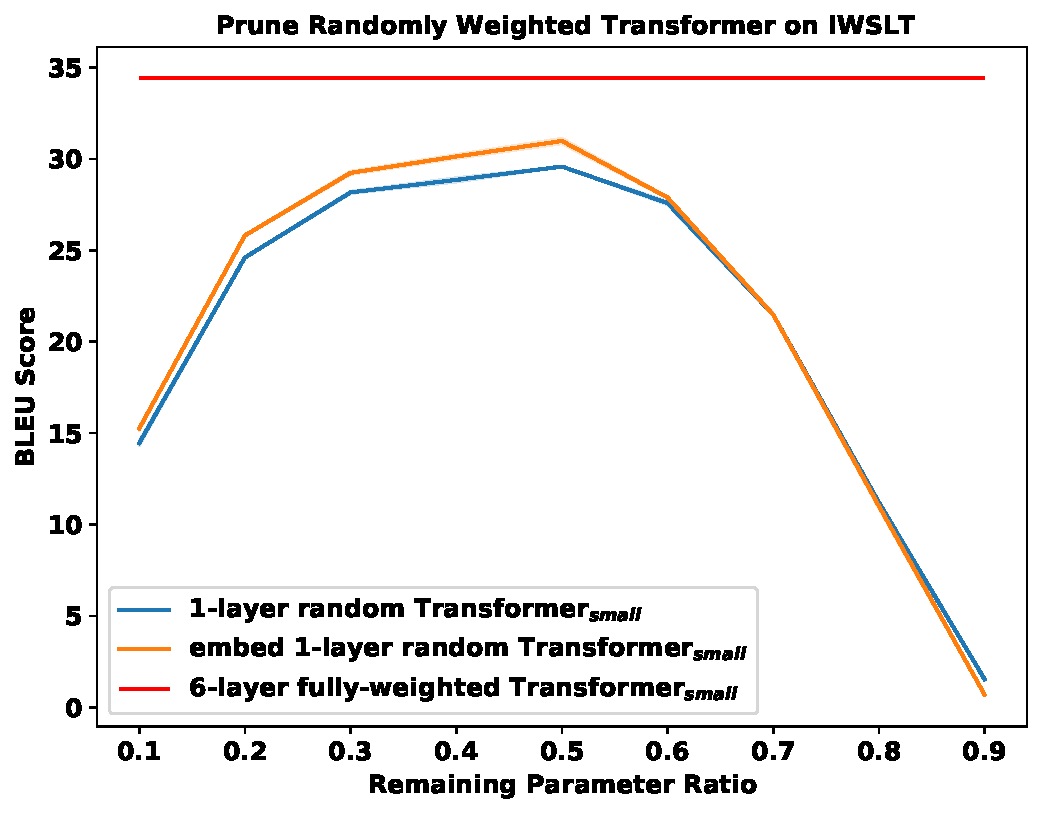
\includegraphics[width=\textwidth]{fig/iwslt_embed.pdf}
    \end{subfigure}
            \vspace{-5pt}
    \caption{The effectiveness of pre-trained embedding layers on WMT14 (left) and IWSLT14 (right).}
    \label{fig:mt_embed}
            \vspace{-10pt}

\end{figure*}

Let us use a toy example to explain why there is no need for $L$ redundant $\rmW_l$s. 
Assume that, for a random weighted matrix $\rmW_l$, the probability that it has a ``good'' subnetwork is $p$\footnote{Here, the ``good'' can be any defined metric, e.g., $(\rmM\odot\rmW_l)\text{x}\approx\rmW^*\text{x}$ for all $x$ and a pre-defined $\rmW^*$.}. 
Furthermore, assume that for two different layers, the probability that both have the ``good'' subnetworks is independent.
Then for $L$ different layers, the probability that all $\rmW_l$s have the ``good'' subnetworks is $p^L$. 
Meanwhile, since $\rmW_1$ has the same initialization method as $\rmW_l$, the probability that $\rmW_1$ has a ``good'' subnetwork for $l$-th layer is also $p$.
Thus, for $L$ different layers, the probability that using $\rmW_1$ to generate all ``good'' subnetworks is also $p^L$. 

In this paper, we investigate the scenario where one randomized layer is applied for $L$ times repeatedly with $L$ different Supermasks. 
As a result, this can reduce the memory footprint since all Supermasks can be stored in the binary format. 


\section{Conclusions}
\label{sec:conclusions}
In this paper, we validate the existence of effective subnetworks in a one-layer randomly weighted Transformer on translation tasks. 
Hidden within a one-layer randomly weighted Transformer$_\text{wide/wider}$ with fixed pre-trained embedding layers, we find there exist subnetworks that are smaller than, but can competitively match, the performance of a trained Transformer$_\text{small/base}$ on IWSLT14/WMT14. 



% \section*{Ethical Considerations}
% One caveat of the proposed method is that data collected from public available resources that may contain biases, toxic contents, and other ethical issues. 
% This problem is common to AI models and we stress that de-biasing and a detailed examination are needed before deploying the system.
\section*{Acknowledgements}
We thank anonymous reviewers for their comments and suggestions. SS and KK were supported by grants from Samsung, Facebook, and the Berkeley Deep Drive Consortium. We would like to acknowledge DARPA, IARPA, NSF, and ONR for providing partial support of this work.
\vspace{-2mm}
\section{Introduction}
\label{sec:intro}
\vspace{-1mm}

Modern deep learning often trains millions or even billions of parameters~\citep{Devlin:2018bert,shoeybi2019megatron,raffel2019exploring,brown2020language} to deliver good performance for a model. 
Recently, \citet{frankle2018lottery,frankle2020linear} demonstrated that these over-parameterized  networks contain sparse subnetworks, when trained in isolation, that can achieve similar or better performance than the original~model.

Furthermore, recent studies revisit the initialization stage of finding these subnetworks in vision models~\citep{Zhou:2019deconstructing,Ramanujan:2020hidden}.
Such a mask, which is used to mask out a part of the entire network to those subnetworks, is referred to as a ``Supermask.'' 
That is to say, subnetworks of a \textit{randomly weighted neural network} (NN) can achieve competitive performance, which may act as a good  ``prior''~\citep{gaier2019weight} and connect to the long history of leveraging random features~\citep{Gamba:1961papa,Baum:1988jc} and/or random kernel methods~\citep{Rahimi:2008random,Rahimi:2009kitchen} in machine learning. 
Here, we examine the following question: how does a fully randomized natural language processing (NLP) model perform in the multi-layer setting, and particularly in the (so far under-explored) one-layer setting?

\begin{figure}
    \centering
    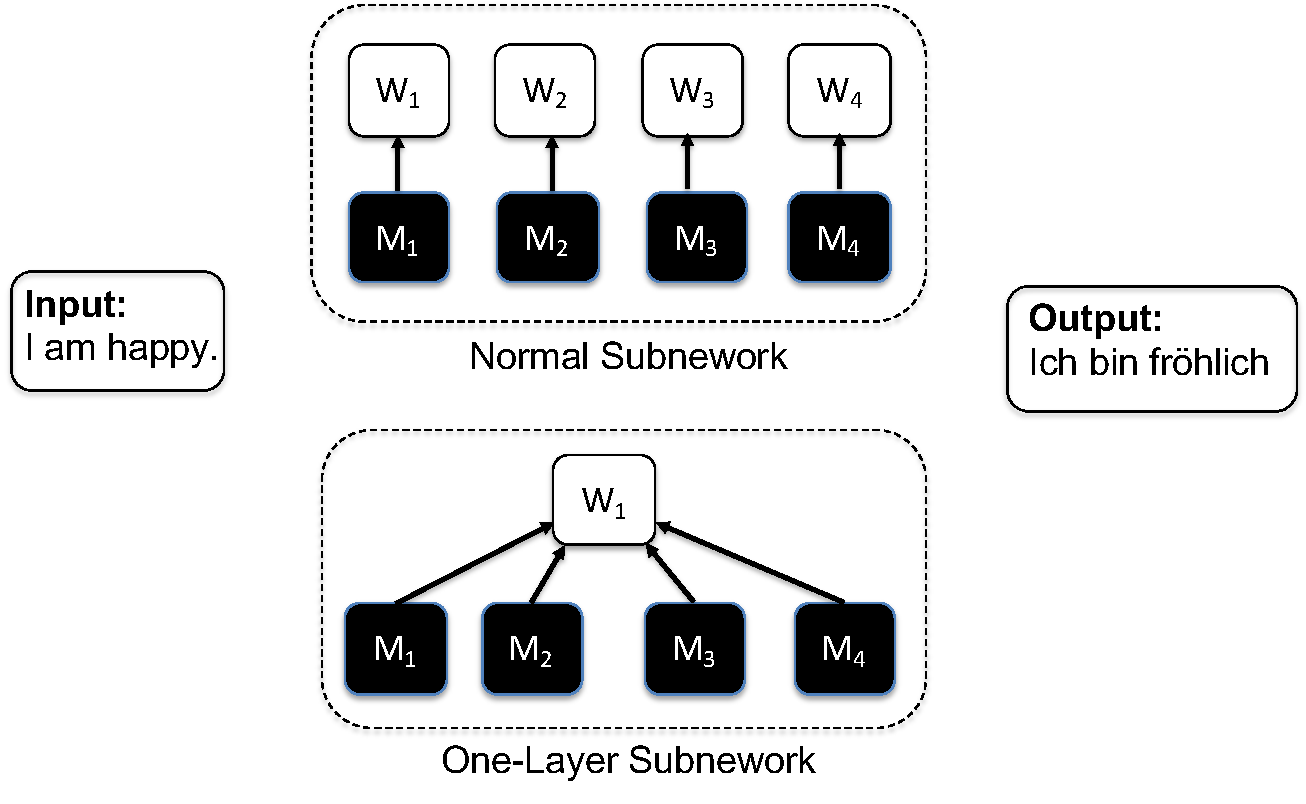
\includegraphics[width=0.8\linewidth]{fig/sketch.pdf}
            \vspace{-5pt}
    \caption{ Illustration plot for a normal subnetwork and a one-layer subnetwork.}
    \label{fig:model_illustration}
    \vspace{-6mm}
\end{figure}

In this work, we first validate that there exist subnetworks of standard randomly weighted Transformers (Reservoir Transformers in~\citep{shen2020reservoir}) that can perform competitively with fully-weighted alternatives on machine translation and natural language understanding tasks. 
With 50\% randomized weights remaining, we found a subnetwork that can reach 29.45/17.29 BLEU on IWSLT14/WMT14, respectively. 
We also investigate the special case of finding subnetworks in one-layer randomly weighted Transformers (see~\fref{fig:model_illustration}). 
To obtain the subnetworks, we repeatedly apply the same randomized Transformer layer several times with different Supermasks. 
The resulting subnetwork of a one-layer randomly-weighted Transformer has similar performance as the multi-layer counterparts with a 30\% lower memory footprint. 
We also study the impact of different depths/widths of Transformers along with the effectiveness of two initialization methods. 
Finally, using the pre-trained embedding layers, we find that the subnetworks hidden in one layer randomly weighted Transformer$_\text{wide/wider}$ are smaller than, but can match 98\%/92\% of the performance of, a trained Transformer$_\text{small/base}$ on IWSLT14/WMT14. 
We hope our findings can offer new insights for understanding Transformers. 
% \vspace{-3mm}
\section{Related Work}
\vspace{-1mm}
\noindent\textbf{Lottery Tickets Hypothesis.}
\citet{frankle2018lottery} found that NNs for computer vision contain subnetworks that can be effectively trained from scratch when reset to their initialization.
Subsequent works~\citep{Zhou:2019deconstructing,Ramanujan:2020hidden,wortsman2020supermasks} demonstrated that so-called winning tickets can achieve performance without training, where the mask for finding the subnetwork at initialization is called ``supermask.'' 
In NLP, previous works find that matching subnetworks exist early in training with Transformers~\citep{yu2019playing}, LSTMs~\citep{renda2020comparing}, and fully-weighted per-trained BERT~\citep{chen2020lottery,prasanna2020bert} or Vison-and-Language model~\citep{gan2021playing}, but not at \textit{initialization}. 

\noindent\textbf{Random Feature.} 
In the early days of neural networks, fixed random layers~\citep{Baum:1988jc,Schmidt:1992pr,Pao:1994nc} have been studied in reservoir computing~\citep{Maass:2002lsm,Jaeger:2003echostate,Lukovsevivcius:2009reservoir}, ``random kitchen sink'' kernel machines~\citep{Rahimi:2008random,Rahimi:2009kitchen}, and so on. 
Recently, random features have also been extensively explored for modern neural networks in deep reservoir computing networks \citep{Scardapane:2017randomness,Gallicchio:2017echo,shen2020reservoir}, random kernel feature~\citep{peng2021random,Choromanski:2020performer}, and  applications in text classification~\citep{Conneau:2017infersent,Wieting:2019notraining}, summarization \citep{Pilault:2020impressive} and probing \citep{voita2020information}. 

\noindent\textbf{Compressing Transformer.} A wide range of neural network compression techniques have been applied to Transformers. 
This includes pruning  \citep{fan2019reducing,michel2019sixteen,sanh2020movement,yao2021mlpruning} where parts of the model weights are dropped, parameter-sharing \citep{lan2020albert,dehghani2018universal,bai2019deep} where the same
parameters are used in different parts of a model, quantization \citep{shen2020q,li2020train}
where the weights of the Transformer model are represented with fewer bits, and distilliation \citep{sun2020mobilebert,jiao2020tinybert} where a compact student model is trained to mimic a larger teacher model. 
To find the proposed subnetwork at initialization, we develop our method in the spirit of parameter sharing and pruning. 

\usepackage[utf8]{inputenc} % allow utf-8 input
\usepackage[T1]{fontenc}    % use 8-bit T1 fonts
\usepackage{url}            % simple URL typesetting
\usepackage{booktabs}       % professional-quality tables
\usepackage{amsfonts}       % blackboard math symbols
\usepackage{nicefrac}       % compact symbols for 1/2, etc.
\usepackage{microtype}      % microtypography
\usepackage{times}
\usepackage{soul}
\usepackage[utf8]{inputenc}
\usepackage{graphicx}
\usepackage{amsmath}
\usepackage{booktabs}
\usepackage{adjustbox}




% \usepackage[colorlinks=true,
% citecolor=blue,
% filecolor=black,
% linkcolor=blue,
% urlcolor=blue]{hyperref}

\usepackage{graphicx}
\usepackage{subfigure}
\usepackage{booktabs} % for professional tables


% Optional math commands from https://github.com/goodfeli/dlbook_notation.
% %%%%% NEW MATH DEFINITIONS %%%%%

\usepackage{amsmath,amsfonts,bm}

% Mark sections of captions for referring to divisions of figures
\newcommand{\figleft}{{\em (Left)}}
\newcommand{\figcenter}{{\em (Center)}}
\newcommand{\figright}{{\em (Right)}}
\newcommand{\figtop}{{\em (Top)}}
\newcommand{\figbottom}{{\em (Bottom)}}
\newcommand{\captiona}{{\em (a)}}
\newcommand{\captionb}{{\em (b)}}
\newcommand{\captionc}{{\em (c)}}
\newcommand{\captiond}{{\em (d)}}

% Highlight a newly defined term
\newcommand{\newterm}[1]{{\bf #1}}


% Figure reference, lower-case.
\def\figref#1{figure~\ref{#1}}
% Figure reference, capital. For start of sentence
\def\Figref#1{Figure~\ref{#1}}
\def\twofigref#1#2{figures \ref{#1} and \ref{#2}}
\def\quadfigref#1#2#3#4{figures \ref{#1}, \ref{#2}, \ref{#3} and \ref{#4}}
% Section reference, lower-case.
\def\secref#1{section~\ref{#1}}
% Section reference, capital.
\def\Secref#1{Section~\ref{#1}}
% Reference to two sections.
\def\twosecrefs#1#2{sections \ref{#1} and \ref{#2}}
% Reference to three sections.
\def\secrefs#1#2#3{sections \ref{#1}, \ref{#2} and \ref{#3}}
% Reference to an equation, lower-case.
\def\eqref#1{equation~\ref{#1}}
% Reference to an equation, upper case
\def\Eqref#1{Equation~\ref{#1}}
% A raw reference to an equation---avoid using if possible
\def\plaineqref#1{\ref{#1}}
% Reference to a chapter, lower-case.
\def\chapref#1{chapter~\ref{#1}}
% Reference to an equation, upper case.
\def\Chapref#1{Chapter~\ref{#1}}
% Reference to a range of chapters
\def\rangechapref#1#2{chapters\ref{#1}--\ref{#2}}
% Reference to an algorithm, lower-case.
\def\algref#1{algorithm~\ref{#1}}
% Reference to an algorithm, upper case.
\def\Algref#1{Algorithm~\ref{#1}}
\def\twoalgref#1#2{algorithms \ref{#1} and \ref{#2}}
\def\Twoalgref#1#2{Algorithms \ref{#1} and \ref{#2}}
% Reference to a part, lower case
\def\partref#1{part~\ref{#1}}
% Reference to a part, upper case
\def\Partref#1{Part~\ref{#1}}
\def\twopartref#1#2{parts \ref{#1} and \ref{#2}}

\def\ceil#1{\lceil #1 \rceil}
\def\floor#1{\lfloor #1 \rfloor}
\def\1{\bm{1}}
\newcommand{\train}{\mathcal{D}}
\newcommand{\valid}{\mathcal{D_{\mathrm{valid}}}}
\newcommand{\test}{\mathcal{D_{\mathrm{test}}}}

\def\eps{{\epsilon}}


% Random variables
\def\reta{{\textnormal{$\eta$}}}
\def\ra{{\textnormal{a}}}
\def\rb{{\textnormal{b}}}
\def\rc{{\textnormal{c}}}
\def\rd{{\textnormal{d}}}
\def\re{{\textnormal{e}}}
\def\rf{{\textnormal{f}}}
\def\rg{{\textnormal{g}}}
\def\rh{{\textnormal{h}}}
\def\ri{{\textnormal{i}}}
\def\rj{{\textnormal{j}}}
\def\rk{{\textnormal{k}}}
\def\rl{{\textnormal{l}}}
% rm is already a command, just don't name any random variables m
\def\rn{{\textnormal{n}}}
\def\ro{{\textnormal{o}}}
\def\rp{{\textnormal{p}}}
\def\rq{{\textnormal{q}}}
\def\rr{{\textnormal{r}}}
\def\rs{{\textnormal{s}}}
\def\rt{{\textnormal{t}}}
\def\ru{{\textnormal{u}}}
\def\rv{{\textnormal{v}}}
\def\rw{{\textnormal{w}}}
\def\rx{{\textnormal{x}}}
\def\ry{{\textnormal{y}}}
\def\rz{{\textnormal{z}}}

% Random vectors
\def\rvepsilon{{\mathbf{\epsilon}}}
\def\rvtheta{{\mathbf{\theta}}}
\def\rva{{\mathbf{a}}}
\def\rvb{{\mathbf{b}}}
\def\rvc{{\mathbf{c}}}
\def\rvd{{\mathbf{d}}}
\def\rve{{\mathbf{e}}}
\def\rvf{{\mathbf{f}}}
\def\rvg{{\mathbf{g}}}
\def\rvh{{\mathbf{h}}}
\def\rvu{{\mathbf{i}}}
\def\rvj{{\mathbf{j}}}
\def\rvk{{\mathbf{k}}}
\def\rvl{{\mathbf{l}}}
\def\rvm{{\mathbf{m}}}
\def\rvn{{\mathbf{n}}}
\def\rvo{{\mathbf{o}}}
\def\rvp{{\mathbf{p}}}
\def\rvq{{\mathbf{q}}}
\def\rvr{{\mathbf{r}}}
\def\rvs{{\mathbf{s}}}
\def\rvt{{\mathbf{t}}}
\def\rvu{{\mathbf{u}}}
\def\rvv{{\mathbf{v}}}
\def\rvw{{\mathbf{w}}}
\def\rvx{{\mathbf{x}}}
\def\rvy{{\mathbf{y}}}
\def\rvz{{\mathbf{z}}}

% Elements of random vectors
\def\erva{{\textnormal{a}}}
\def\ervb{{\textnormal{b}}}
\def\ervc{{\textnormal{c}}}
\def\ervd{{\textnormal{d}}}
\def\erve{{\textnormal{e}}}
\def\ervf{{\textnormal{f}}}
\def\ervg{{\textnormal{g}}}
\def\ervh{{\textnormal{h}}}
\def\ervi{{\textnormal{i}}}
\def\ervj{{\textnormal{j}}}
\def\ervk{{\textnormal{k}}}
\def\ervl{{\textnormal{l}}}
\def\ervm{{\textnormal{m}}}
\def\ervn{{\textnormal{n}}}
\def\ervo{{\textnormal{o}}}
\def\ervp{{\textnormal{p}}}
\def\ervq{{\textnormal{q}}}
\def\ervr{{\textnormal{r}}}
\def\ervs{{\textnormal{s}}}
\def\ervt{{\textnormal{t}}}
\def\ervu{{\textnormal{u}}}
\def\ervv{{\textnormal{v}}}
\def\ervw{{\textnormal{w}}}
\def\ervx{{\textnormal{x}}}
\def\ervy{{\textnormal{y}}}
\def\ervz{{\textnormal{z}}}

% Random matrices
\def\rmA{{\mathbf{A}}}
\def\rmB{{\mathbf{B}}}
\def\rmC{{\mathbf{C}}}
\def\rmD{{\mathbf{D}}}
\def\rmE{{\mathbf{E}}}
\def\rmF{{\mathbf{F}}}
\def\rmG{{\mathbf{G}}}
\def\rmH{{\mathbf{H}}}
\def\rmI{{\mathbf{I}}}
\def\rmJ{{\mathbf{J}}}
\def\rmK{{\mathbf{K}}}
\def\rmL{{\mathbf{L}}}
\def\rmM{{\mathbf{M}}}
\def\rmN{{\mathbf{N}}}
\def\rmO{{\mathbf{O}}}
\def\rmP{{\mathbf{P}}}
\def\rmQ{{\mathbf{Q}}}
\def\rmR{{\mathbf{R}}}
\def\rmS{{\mathbf{S}}}
\def\rmT{{\mathbf{T}}}
\def\rmU{{\mathbf{U}}}
\def\rmV{{\mathbf{V}}}
\def\rmW{{\mathbf{W}}}
\def\rmX{{\mathbf{X}}}
\def\rmY{{\mathbf{Y}}}
\def\rmZ{{\mathbf{Z}}}

% Elements of random matrices
\def\ermA{{\textnormal{A}}}
\def\ermB{{\textnormal{B}}}
\def\ermC{{\textnormal{C}}}
\def\ermD{{\textnormal{D}}}
\def\ermE{{\textnormal{E}}}
\def\ermF{{\textnormal{F}}}
\def\ermG{{\textnormal{G}}}
\def\ermH{{\textnormal{H}}}
\def\ermI{{\textnormal{I}}}
\def\ermJ{{\textnormal{J}}}
\def\ermK{{\textnormal{K}}}
\def\ermL{{\textnormal{L}}}
\def\ermM{{\textnormal{M}}}
\def\ermN{{\textnormal{N}}}
\def\ermO{{\textnormal{O}}}
\def\ermP{{\textnormal{P}}}
\def\ermQ{{\textnormal{Q}}}
\def\ermR{{\textnormal{R}}}
\def\ermS{{\textnormal{S}}}
\def\ermT{{\textnormal{T}}}
\def\ermU{{\textnormal{U}}}
\def\ermV{{\textnormal{V}}}
\def\ermW{{\textnormal{W}}}
\def\ermX{{\textnormal{X}}}
\def\ermY{{\textnormal{Y}}}
\def\ermZ{{\textnormal{Z}}}

% Vectors
\def\vzero{{\bm{0}}}
\def\vone{{\bm{1}}}
\def\vmu{{\bm{\mu}}}
\def\vtheta{{\bm{\theta}}}
\def\va{{\bm{a}}}
\def\vb{{\bm{b}}}
\def\vc{{\bm{c}}}
\def\vd{{\bm{d}}}
\def\ve{{\bm{e}}}
\def\vf{{\bm{f}}}
\def\vg{{\bm{g}}}
\def\vh{{\bm{h}}}
\def\vi{{\bm{i}}}
\def\vj{{\bm{j}}}
\def\vk{{\bm{k}}}
\def\vl{{\bm{l}}}
\def\vm{{\bm{m}}}
\def\vn{{\bm{n}}}
\def\vo{{\bm{o}}}
\def\vp{{\bm{p}}}
\def\vq{{\bm{q}}}
\def\vr{{\bm{r}}}
\def\vs{{\bm{s}}}
\def\vt{{\bm{t}}}
\def\vu{{\bm{u}}}
\def\vv{{\bm{v}}}
\def\vw{{\bm{w}}}
\def\vx{{\bm{x}}}
\def\vy{{\bm{y}}}
\def\vz{{\bm{z}}}

% Elements of vectors
\def\evalpha{{\alpha}}
\def\evbeta{{\beta}}
\def\evepsilon{{\epsilon}}
\def\evlambda{{\lambda}}
\def\evomega{{\omega}}
\def\evmu{{\mu}}
\def\evpsi{{\psi}}
\def\evsigma{{\sigma}}
\def\evtheta{{\theta}}
\def\eva{{a}}
\def\evb{{b}}
\def\evc{{c}}
\def\evd{{d}}
\def\eve{{e}}
\def\evf{{f}}
\def\evg{{g}}
\def\evh{{h}}
\def\evi{{i}}
\def\evj{{j}}
\def\evk{{k}}
\def\evl{{l}}
\def\evm{{m}}
\def\evn{{n}}
\def\evo{{o}}
\def\evp{{p}}
\def\evq{{q}}
\def\evr{{r}}
\def\evs{{s}}
\def\evt{{t}}
\def\evu{{u}}
\def\evv{{v}}
\def\evw{{w}}
\def\evx{{x}}
\def\evy{{y}}
\def\evz{{z}}

% Matrix
\def\mA{{\bm{A}}}
\def\mB{{\bm{B}}}
\def\mC{{\bm{C}}}
\def\mD{{\bm{D}}}
\def\mE{{\bm{E}}}
\def\mF{{\bm{F}}}
\def\mG{{\bm{G}}}
\def\mH{{\bm{H}}}
\def\mI{{\bm{I}}}
\def\mJ{{\bm{J}}}
\def\mK{{\bm{K}}}
\def\mL{{\bm{L}}}
\def\mM{{\bm{M}}}
\def\mN{{\bm{N}}}
\def\mO{{\bm{O}}}
\def\mP{{\bm{P}}}
\def\mQ{{\bm{Q}}}
\def\mR{{\bm{R}}}
\def\mS{{\bm{S}}}
\def\mT{{\bm{T}}}
\def\mU{{\bm{U}}}
\def\mV{{\bm{V}}}
\def\mW{{\bm{W}}}
\def\mX{{\bm{X}}}
\def\mY{{\bm{Y}}}
\def\mZ{{\bm{Z}}}
\def\mBeta{{\bm{\beta}}}
\def\mPhi{{\bm{\Phi}}}
\def\mLambda{{\bm{\Lambda}}}
\def\mSigma{{\bm{\Sigma}}}

% Tensor
\DeclareMathAlphabet{\mathsfit}{\encodingdefault}{\sfdefault}{m}{sl}
\SetMathAlphabet{\mathsfit}{bold}{\encodingdefault}{\sfdefault}{bx}{n}
\newcommand{\tens}[1]{\bm{\mathsfit{#1}}}
\def\tA{{\tens{A}}}
\def\tB{{\tens{B}}}
\def\tC{{\tens{C}}}
\def\tD{{\tens{D}}}
\def\tE{{\tens{E}}}
\def\tF{{\tens{F}}}
\def\tG{{\tens{G}}}
\def\tH{{\tens{H}}}
\def\tI{{\tens{I}}}
\def\tJ{{\tens{J}}}
\def\tK{{\tens{K}}}
\def\tL{{\tens{L}}}
\def\tM{{\tens{M}}}
\def\tN{{\tens{N}}}
\def\tO{{\tens{O}}}
\def\tP{{\tens{P}}}
\def\tQ{{\tens{Q}}}
\def\tR{{\tens{R}}}
\def\tS{{\tens{S}}}
\def\tT{{\tens{T}}}
\def\tU{{\tens{U}}}
\def\tV{{\tens{V}}}
\def\tW{{\tens{W}}}
\def\tX{{\tens{X}}}
\def\tY{{\tens{Y}}}
\def\tZ{{\tens{Z}}}


% Graph
\def\gA{{\mathcal{A}}}
\def\gB{{\mathcal{B}}}
\def\gC{{\mathcal{C}}}
\def\gD{{\mathcal{D}}}
\def\gE{{\mathcal{E}}}
\def\gF{{\mathcal{F}}}
\def\gG{{\mathcal{G}}}
\def\gH{{\mathcal{H}}}
\def\gI{{\mathcal{I}}}
\def\gJ{{\mathcal{J}}}
\def\gK{{\mathcal{K}}}
\def\gL{{\mathcal{L}}}
\def\gM{{\mathcal{M}}}
\def\gN{{\mathcal{N}}}
\def\gO{{\mathcal{O}}}
\def\gP{{\mathcal{P}}}
\def\gQ{{\mathcal{Q}}}
\def\gR{{\mathcal{R}}}
\def\gS{{\mathcal{S}}}
\def\gT{{\mathcal{T}}}
\def\gU{{\mathcal{U}}}
\def\gV{{\mathcal{V}}}
\def\gW{{\mathcal{W}}}
\def\gX{{\mathcal{X}}}
\def\gY{{\mathcal{Y}}}
\def\gZ{{\mathcal{Z}}}

% Sets
\def\sA{{\mathbb{A}}}
\def\sB{{\mathbb{B}}}
\def\sC{{\mathbb{C}}}
\def\sD{{\mathbb{D}}}
% Don't use a set called E, because this would be the same as our symbol
% for expectation.
\def\sF{{\mathbb{F}}}
\def\sG{{\mathbb{G}}}
\def\sH{{\mathbb{H}}}
\def\sI{{\mathbb{I}}}
\def\sJ{{\mathbb{J}}}
\def\sK{{\mathbb{K}}}
\def\sL{{\mathbb{L}}}
\def\sM{{\mathbb{M}}}
\def\sN{{\mathbb{N}}}
\def\sO{{\mathbb{O}}}
\def\sP{{\mathbb{P}}}
\def\sQ{{\mathbb{Q}}}
\def\sR{{\mathbb{R}}}
\def\sS{{\mathbb{S}}}
\def\sT{{\mathbb{T}}}
\def\sU{{\mathbb{U}}}
\def\sV{{\mathbb{V}}}
\def\sW{{\mathbb{W}}}
\def\sX{{\mathbb{X}}}
\def\sY{{\mathbb{Y}}}
\def\sZ{{\mathbb{Z}}}

% Entries of a matrix
\def\emLambda{{\Lambda}}
\def\emA{{A}}
\def\emB{{B}}
\def\emC{{C}}
\def\emD{{D}}
\def\emE{{E}}
\def\emF{{F}}
\def\emG{{G}}
\def\emH{{H}}
\def\emI{{I}}
\def\emJ{{J}}
\def\emK{{K}}
\def\emL{{L}}
\def\emM{{M}}
\def\emN{{N}}
\def\emO{{O}}
\def\emP{{P}}
\def\emQ{{Q}}
\def\emR{{R}}
\def\emS{{S}}
\def\emT{{T}}
\def\emU{{U}}
\def\emV{{V}}
\def\emW{{W}}
\def\emX{{X}}
\def\emY{{Y}}
\def\emZ{{Z}}
\def\emSigma{{\Sigma}}

% entries of a tensor
% Same font as tensor, without \bm wrapper
\newcommand{\etens}[1]{\mathsfit{#1}}
\def\etLambda{{\etens{\Lambda}}}
\def\etA{{\etens{A}}}
\def\etB{{\etens{B}}}
\def\etC{{\etens{C}}}
\def\etD{{\etens{D}}}
\def\etE{{\etens{E}}}
\def\etF{{\etens{F}}}
\def\etG{{\etens{G}}}
\def\etH{{\etens{H}}}
\def\etI{{\etens{I}}}
\def\etJ{{\etens{J}}}
\def\etK{{\etens{K}}}
\def\etL{{\etens{L}}}
\def\etM{{\etens{M}}}
\def\etN{{\etens{N}}}
\def\etO{{\etens{O}}}
\def\etP{{\etens{P}}}
\def\etQ{{\etens{Q}}}
\def\etR{{\etens{R}}}
\def\etS{{\etens{S}}}
\def\etT{{\etens{T}}}
\def\etU{{\etens{U}}}
\def\etV{{\etens{V}}}
\def\etW{{\etens{W}}}
\def\etX{{\etens{X}}}
\def\etY{{\etens{Y}}}
\def\etZ{{\etens{Z}}}

% The true underlying data generating distribution
\newcommand{\pdata}{p_{\rm{data}}}
% The empirical distribution defined by the training set
\newcommand{\ptrain}{\hat{p}_{\rm{data}}}
\newcommand{\Ptrain}{\hat{P}_{\rm{data}}}
% The model distribution
\newcommand{\pmodel}{p_{\rm{model}}}
\newcommand{\Pmodel}{P_{\rm{model}}}
\newcommand{\ptildemodel}{\tilde{p}_{\rm{model}}}
% Stochastic autoencoder distributions
\newcommand{\pencode}{p_{\rm{encoder}}}
\newcommand{\pdecode}{p_{\rm{decoder}}}
\newcommand{\precons}{p_{\rm{reconstruct}}}

\newcommand{\laplace}{\mathrm{Laplace}} % Laplace distribution

\newcommand{\E}{\mathbb{E}}
\newcommand{\Ls}{\mathcal{L}}
\newcommand{\R}{\mathbb{R}}
\newcommand{\emp}{\tilde{p}}
\newcommand{\lr}{\alpha}
\newcommand{\reg}{\lambda}
\newcommand{\rect}{\mathrm{rectifier}}
\newcommand{\softmax}{\mathrm{softmax}}
\newcommand{\sigmoid}{\sigma}
\newcommand{\softplus}{\zeta}
\newcommand{\KL}{D_{\mathrm{KL}}}
\newcommand{\Var}{\mathrm{Var}}
\newcommand{\standarderror}{\mathrm{SE}}
\newcommand{\Cov}{\mathrm{Cov}}
% Wolfram Mathworld says $L^2$ is for function spaces and $\ell^2$ is for vectors
% But then they seem to use $L^2$ for vectors throughout the site, and so does
% wikipedia.
\newcommand{\normlzero}{L^0}
\newcommand{\normlone}{L^1}
\newcommand{\normltwo}{L^2}
\newcommand{\normlp}{L^p}
\newcommand{\normmax}{L^\infty}

\newcommand{\parents}{Pa} % See usage in notation.tex. Chosen to match Daphne's book.

\DeclareMathOperator*{\argmax}{arg\,max}
\DeclareMathOperator*{\argmin}{arg\,min}

\DeclareMathOperator{\sign}{sign}
\DeclareMathOperator{\Tr}{Tr}
\let\ab\allowbreak


\usepackage{multirow}
\usepackage{paralist}

\usepackage{booktabs} % for professional tables
\usepackage{multicol}
\usepackage{diagbox}

\usepackage[ruled,noend]{algorithm2e}
\newcommand{\theHalgorithm}{\arabic{algorithm}}
\newcommand\mycommfont[1]{\scriptsize\ttfamily\textcolor{blue}{#1}}
\SetCommentSty{mycommfont}

\usepackage{here}

\usepackage{amsmath,amssymb,amsfonts,amsbsy,amsfonts,latexsym}
\usepackage{multirow}
\usepackage{makecell}
% \usepackage[labelfont=bf,textfont=it,belowskip=0pt,aboveskip=5pt,tableposition=top]{caption}
\usepackage{xcolor}
\usepackage{colortbl}
\let\proof\relax
\let\endproof\relax


\definecolor{colorA}{RGB}{189,201,225}
\definecolor{colorB}{RGB}{103,169,207}
\definecolor{colorC}{RGB}{ 28,144,153}
\definecolor{colorD}{RGB}{  1,108, 89}

\newcolumntype{R}{>{\columncolor{gray!40}}r}
\newcolumntype{L}{>{\columncolor{gray!40}}l}
\newcolumntype{C}{>{\columncolor{gray!40}}c}
\newcommand{\highlightrow}{\rowcolor{orange!20}}




%table
\usepackage{tabularx,colortbl,xcolor}
\usepackage{multirow}
\usepackage[normalem]{ulem}
\useunder{\uline}{\ul}{}

\newcommand\hy{\textrm{-}}

\usepackage{enumitem}

\usepackage{xparse}% http://ctan.org/pkg/xparse

% \captionsetup[table]{name=Table}
\DeclareGraphicsExtensions{.pdf,.png}


\SetKwInput{KwInput}{Input}
\newcommand{\pluseq}{\mathrel{+}=}
\newcommand{\asteq}{\mathrel{*}=}
\newcommand{\diveq}{\mathrel{/}=}

\usepackage{longtable}
% \usepackage{pgfplots}

\usepackage{url}
\usepackage{booktabs}
\usepackage{multirow}
\usepackage{array, caption, makecell, booktabs}
\usepackage{wrapfig}
% \usepackage{floatrow}
\usepackage{comment}
\usepackage{enumitem}
\usepackage{accents}
